\section{Equazioni Differenziali Ordinarie}
\begin{definition}[EDO di ordine $n$]
    Un'equazione differenziale ordinaria di ordine $n$ è un'equazione della forma
    \begin{equation}\label{eq:EDO}
        F(x,y,y', y'', \hdots, y^{(n)})=0,
    \end{equation}
    dove $F\colon U\subseteq\mathbb R^{n+2}\rightarrow\mathbb R$ e $y=y(x)\colon\mathbb R\rightarrow\mathbb R$ funzione incognita.
    \begin{align*}
        F\colon U\subseteq\mathbb R^{n+2} & \rightarrow\mathbb R\\
        x,y,y',\hdots, y^{(n)} & \mapsto F(x,y,y', \hdots, y^{(n)}).
    \end{align*}
\end{definition}

\begin{definition}[EDO ordinaria]
    Una EDO è ordinaria in quanto l'incognita è una funzione di una variabile.
\end{definition}

Nel caso in cui l'incognita dipenda da più variabili allora non è una EDO ma un'equazione differenziale alle derivate parziali.

\begin{definition}[Ordine di una EDO]
    L'ordine di una EDO è l'ordine massimo di derivazione che compare nell'equazione.
\end{definition}

La definizione di ordine di una EDO può essere trasformata in "$y$ può essere derivata $n$ volte".

\begin{example}[EDO lineare di ordine 3]
    $xy'''+5y=\sin x$. $y'''$ è la derivata terza di $y$.
\end{example}

L'obiettivo è trovare una soluzione all'equazione (\ref{eq:EDO}).

\begin{definition}[Soluzione di una EDO]\label{def:curva_integrale_EDO}
    Una soluzione (o soluzione a curva integrale) di (\ref{eq:EDO}) sull'intervallo $I\subseteq\mathbb R$ è una funzione $\varphi=\varphi(x)$, con $x\in I$, definita e differenziabile $n$ volte su $I$ tale che
    \begin{equation*}
        \varphi(x),\varphi'(x),\hdots,\varphi^{(n)}(x)\in U\subseteq\mathbb R^{(n+2)},\quad \forall x\in I=[a,b]
    \end{equation*}
    e
    \begin{equation*}
        F(x,\varphi(x),\varphi'(x),\hdots,\varphi^{(n)})=0.
    \end{equation*}
\end{definition}

\paragraph{N.B.:} $\varphi$ è definita su un intervallo non disgiunto, ovvero è definita su un intervallo che non ha salti del tipo $[0,1)\cup[2, +\infty)$.

\begin{definition}[Integrale generale]\label{def:integrale_generale_EDO}
    L'integrale generale della EDO (\ref{eq:EDO}), definita su $I=[a,b]\subseteq \mathbb R$, è l'insieme di tutte le soluzioni dell'EDO in $I$.
\end{definition}

L'integrale generale è l'insieme di tutte le soluzioni $\varphi$.

Sarà utile il concetto di primitiva di una funzione $f(x)$. La sua definizione è quella di Analisi 1, ovvero la seguente.

\begin{definition}[Primitiva]
    Sia $f\colon (a,b)\rightarrow\mathbb R$. La funzione $y(x)$ è una primitiva di $f$ in $(a,b)$ se è derivabile in $(a,b)$ e se
    \begin{equation*}
        y'(x)=f(x)\quad\forall x\in(a,b).
    \end{equation*}
\end{definition}

La funzione $y(x)$ è una EDO di primo ordine.

Una conseguenza del Teorema Fondamentale del Calcolo è la seguente osservazione:
\begin{remark}
    Data $f\colon\mathbb R \rightarrow \mathbb R$, l'integrale generale di una EDO del tipo (\ref{eq:EDO}) è
    \begin{equation}\label{eq:primitiva}
        y(x)=y(x,c)=\int f(x) dx+c\quad c\in\mathbb R.
    \end{equation}
\end{remark} 

L'integrale generale di una EDO denotato come $y(x,c)$, il quale rappresenta le infinite soluzioni (per il valore $c$) per (\ref{eq:EDO}) ed una famiglia di soluzioni dipendenti da una costante ed una variabile indipendente ($c$ e $x$).

\begin{definition}[EDO in forma normale]
    Una EDO del tipo (\ref{eq:EDO}) è in forma normale se nella forma
    \begin{equation}\label{eq:EDO_forma_normale}
        y^{(n)}(x)=\underbrace{f(x, y(x), y'(x),\hdots,y^{(n-1)}(x))}_{F(x, y, y',\hdots, y^{(n-1)})}, \quad f\colon I\in\subseteq\mathbb R^{n}\rightarrow\mathbb R.
    \end{equation}
\end{definition}

In questo caso la EDO è esplicitata rispetto alla derivata di ordine più alto.

Per trovare la soluzione della EDO è necessario stare attenti alle ipotesi del secondo membro, ovvero le ipotesi che verificano $f$. Fatte le opportune ipotesi è possibile dimostrare che per questo problema esiste un'unica soluzione. La soluzione sarà definita localmente in un intervallo di $x_0$ (variabile reale), sotto la condizione iniziale (vedere Problema di Cauchy, Sezione \ref{ssec:problema_cauchy}).

\begin{example}
    $y^{(7)}(x)=5y'+44\tan x$ è una EDO di ordine 7 in forma normale.
\end{example}
\begin{definition}[EDO lineare di ordine $n$]
    Una EDO del tipo (\ref{eq:EDO}) è lineare se nella forma
    \begin{equation}\label{eq:EDO_lineare_ordine_n}
        a_n(x)y^{(n)}(x)+a_{n-1}(x)y^{(n-1)}(x)+\hdots+a_1(x)y'(x)+a_0(x)y(x)=f(x),
    \end{equation}
    dove $a_0(x),a_1(x),\hdots, a_n(x)$, dette funzioni coefficienti dell'equazione, e  $f(x)$, detta termine noto dell'equazione, sono funzioni assegnate, definite e continue per un intervallo $I=[a,b]$.
\end{definition}

\begin{definition}[EDO lineare di ordine $n$ in forma normale]\label{def:EDO_lineare_completa_ordine_n_forma_normale}\footnote{Slide 10 PDF 1.}
    Una EDO lineare di ordine $n$ in forma normale è definita come
    \begin{equation}\label{eq:EDO_lineare_ordine_n_forma_normale}
        y^{(n)}(x)+a_{n-1}(x)y^{(n-1)}(x)+\hdots+a_1(x)y'(x)+a_0(x)y(x)=f(x),
    \end{equation}
    dove $a_n(x)=1$.
\end{definition}

\begin{definition}[EDO lineare completa]
    Una EDO lineare in forma (\ref{eq:EDO_lineare_ordine_n}) è detta completa quando il termine noto $f(x)$ è diverso da 0.
\end{definition}

\paragraph{N.B.:} Il termine "non omogenea" è sinonimo di "completa".

Una soluzione è l'insieme delle soluzioni all'equazione (\ref{eq:EDO_lineare_ordine_n}), può essere ricondotto alla Definizione \ref{def:curva_integrale_EDO} ed alla Definizione \ref{def:integrale_generale_EDO} per EDO in forma normale (\ref{eq:EDO_forma_normale}).

\begin{example}
    \footnote{Slide 10 PDF 1.} $y'(t)=\frac{(t+y(t))^2}{3t^2}$ è una EDO non lineare di ordine 1. 
\end{example}

\begin{example}
    \footnote{Slide 11 PDF 1.} $y''+5y'+7y=e^x$, dove $a_2(x)=1,\, a_1(x)=5,\, a_0(x)=7$ e $f(x)=e^x$, è una EDO lineare del $2^\circ$ ordine a coefficienti costanti.
\end{example}

\begin{definition}[EDO lineare omogenea associata di ordine $n$]\label{def:EDO_lineare_omogenea_ordine_n}
    L'EDO lineare omogenea associata a (\ref{eq:EDO_lineare_ordine_n}) di ordine $n$ è definita come
    \begin{equation}\label{eq:EDO_lineare_omogenea_associata_ordine_n}
        a_n(x)y^{(n)}(x)+a_{n-1}(x)y^{(n-1)}(x)+\hdots+a_1(x)y'(x)+a_0(x)y(x)=0.
    \end{equation}
\end{definition}

\paragraph{Perché una EDO è detta lineare?} \footnote{Slide 11 PDF 1, PG 98.} Una EDO in forma normale del tipo (\ref{eq:EDO_forma_normale}) è detta lineare perché esiste un'\gls{applicazione lineare} fra spazi di funzioni $L\colon C^n(I)\rightarrow C^0(I)$, detta anche operatore, che associa ad ogni funzione $\varphi\in C^n(I)$ una funzione continua del tipo
\begin{equation*}
    L(\varphi(x)):=a_n(x)\varphi^{(n)}(x)+a_{n-1}(x)\varphi^{(n-1)}(x)+\hdots+a_0(x)\varphi(x).
\end{equation*}
L'\gls{applicazione lineare} $L$ è una somma di funzioni continue ed è lineare in quanto soddisfa la seguente proprietà di additività:
\begin{equation*}
    L(\alpha\varphi_1(x)+\beta\varphi_2(x))=\alpha L(\varphi_1(x)) + \beta L(\varphi_2(x)),\quad\forall \alpha,\beta\in\mathbb R,\, \varphi_1(x),\varphi_2(x)\in C^n(I). \qed
\end{equation*}

\paragraph{Nota:} La linearità di una EDO è utile nella dimostrazione del Teorema \ref{th:rappresentazione_integrale_generale_EDO_lineare} di Rappresentazione dell'integrale generale di una EDO lineare.

Le EDO (\ref{eq:EDO_lineare_ordine_n}) e (\ref{eq:EDO_lineare_omogenea_associata_ordine_n}) sono importanti per il Teorema \ref{th:rappresentazione_integrale_generale_EDO_lineare}. Tale teorema è importante per le EDO lineari di ordine $n$, vale per tutte le EDO di ordine $n\geq 1$ ed enuncia che l'integrale generale della EDO del tipo (\ref{eq:EDO_lineare_ordine_n}) è dato dalla somma dell'integrale generale (una soluzione nota della omogenea) dell'omogenea (\ref{eq:EDO_lineare_omogenea_associata_ordine_n}) e dall'integrale generale (una soluzione particolare) dell'equazione non omogenea (\ref{eq:EDO_lineare_ordine_n}).

\begin{theorem}[Rappresentazione dell'integrale generale di una EDO lineare]\label{th:rappresentazione_integrale_generale_EDO_lineare}\footnote{Slide 1 PDF 2.}
    L'integrale generale di una EDO lineare di ordine $n$ definita su $I$ del tipo (\ref{eq:EDO_lineare_ordine_n}) è dato dalla somma dell'integrale generale della sua omogenea associata del tipo (\ref{eq:EDO_lineare_omogenea_associata_ordine_n}) ed una curva integrale della non omogenea  del tipo(\ref{eq:EDO_lineare_ordine_n}), ovvero:
    \begin{equation}\label{eq:rappresentazione_integrale_generale_EDO_lineare}
        y(x)=z(x)+\overline{y}(x),\quad x\in(a,b),
    \end{equation}
    dove $y(x)$ è una soluzione qualsiasi della EDO lineare di ordine $n$ \footnote{Quindi elemento dell'integrale generale.}, $z(x)$ è una soluzione qualsiasi della EDO lineare omogenea associata di ordine $n$ e $\overline{y}(x)$ una soluzione particolare e nota della EDO lineare di ordine $n$. 
\end{theorem} 

\begin{proof}\footnote{PDF 2, Slide 1.}
    \textbf{Per} $\boldsymbol{n=1}$ \textbf{(valido anche per} $\boldsymbol{n>1)}$. Sia la EDO lineare (\ref{eq:EDO_lineare_ordine_n_forma_normale}) di ordine $n=1$ in forma normale e l'omogenea associata:
    \begin{equation}\label{eq:EDO_lineare_ordine_1_forma_normale}
        y'(x)+a(x)y(x)=f(x),
    \end{equation}
    \begin{equation}\label{eq:EDO_lineare_omogenea_associata_ordine_1_forma_normale}
        y'(x)+a(x)y(x)=0,\quad x\in I=[a,b]
    \end{equation}
    Date $y(x)$ soluzione qualsiasi di (\ref{eq:EDO_lineare_ordine_1_forma_normale}) e $\overline{y}(x)$ una soluzione particolare e nota di (\ref{eq:EDO_lineare_ordine_1_forma_normale}), è necessario mostrare che la differenza
    \begin{equation*}
        z(x)=y(x)-\overline{y}(x)
    \end{equation*}
    è una soluzione particolare della EDO omogenea (\ref{eq:EDO_lineare_omogenea_associata_ordine_1_forma_normale}). Dunque
    \begin{equation*}
        y'(x)+a(x)y(x)=f(x),\quad \overline{y}'(x) +a(x)\overline{y}(x)=f(x),\quad \forall x\in I.
    \end{equation*}
    Sottraendo membro a membro
    \begin{equation*}
        \begin{matrix}
            y'(x)+a(x)y(x) - [\overline{y}'(x) +a(x)\overline{y}(x)] =f(x)-f(x),\\\\
            y'(x) - \overline{y}'(x)+a(x)[y(x)-\overline{y}(x)]=0,\\\\
            [y(x)-\overline{y}(x)]'+a(x)[y(x)-\overline{y}(x)]=0,
        \end{matrix}
    \end{equation*}
    quindi vale (\ref{eq:EDO_lineare_omogenea_associata_ordine_1_forma_normale}).\\
    Denotando $z(x)=y(x)-\overline{y}(x)$, con $x\in(a,b)$, per verificare (\ref{eq:EDO_lineare_omogenea_associata_ordine_1_forma_normale}) è necessario verificare \footnote{Presa una soluzione qualsiasi di (\ref{eq:EDO_lineare_omogenea_associata_ordine_1_forma_normale} ed una soluzione nota di (\ref{eq:EDO_lineare_non_omogenea_primo_ordine_forma_normale}), è necessario verificare che la somma verifichi (\ref{eq:EDO_lineare_non_omogenea_primo_ordine_forma_normale}), ovvero (\ref{eq:da_verificare}).}
    \begin{equation}\label{eq:da_verificare}
        y(x)=z(x)+\overline{y}(x),\quad x\in I=[a,b].
    \end{equation}
    [Ovvero:] Viceversa, se $z(x)$ è una soluzione qualsiasi di (\ref{eq:EDO_lineare_omogenea_associata_ordine_1_forma_normale}) su $[a,b]$ e $\overline{y}(x)$ soluzione particolare (e nota) di (\ref{eq:EDO_lineare_ordine_1_forma_normale}), allora è necessario mostrare che la loro somma
    \begin{equation*}
        y(x)=z(x)+\overline{y}(x)
    \end{equation*}
    è soluzione di (\ref{eq:EDO_lineare_ordine_1_forma_normale}). Infatti
    \begin{equation*}
        \begin{matrix}
            y'(x)&=&[z(x)+\overline{y}(x)]'&=&z'(x)+\overline{y}'(x)-a(x)z(x)-a(x)\overline{y}(x)+f(x) &=& \\\\
            &&&=&[z(x)+\overline{y}(x)]'+a(x)[z(x)+\overline{y}(x)]&=&f(x),
        \end{matrix}
    \end{equation*}
    quindi
    \begin{equation*}
        y'(x)+a(x)y(x)=f(x),\quad \forall x\in I=[a,b],
    \end{equation*}
    ovvero è ottenuto che $y(x)=\overline{y}(x)+z(x)$ è soluzione generale di (\ref{eq:EDO_lineare_ordine_1_forma_normale}).
\end{proof}

\paragraph{Cosa afferma il Teorema \ref{th:rappresentazione_integrale_generale_EDO_lineare} di Rappresentazione dell'integrale di una EDO lineare?} Afferma che il vero problema è trovare l'integrale generale (l'insieme delle soluzioni) dell'omogenea. È possibile individuare la soluzione nota ad occhio oppure con il metodo di somiglianza oppure di variazione delle costanti (vedere Sezioni \ref{ssec:metodo_somiglianza} e \ref{ssec:variazione_costanti}).

\paragraph{Rappresentazione alternativa dell'integrale generale:} L'integrale generale rappresentato in forma (\ref{eq:rappresentazione_integrale_generale_EDO_lineare}) può essere visto in modo informale come
\begin{equation*}
\int \text{ generale di (\ref{eq:EDO_lineare_ordine_n})}=\int{\text{ generale di (\ref{eq:EDO_lineare_omogenea_associata_ordine_n})}} + \int\text{ particolare di (\ref{eq:EDO_lineare_ordine_n})}.
\end{equation*}

Ovvero, per trovare tutte le soluzioni della EDO lineare è necessario sommare tutte le soluzioni omogenee e la soluzione nota dell'equazione di partenza.

\paragraph{Passi da fare per trovare l'integrale generale di una EDO lineare di ordine $\boldsymbol n$:} \textbf{Per trovare l'integrale generale di (\ref{eq:EDO_lineare_ordine_n}), è necessario:
\begin{enumerate}
    \item trasformare la EDO in forma normale,
    \item trovare la soluzione della EDO omogenea (\ref{eq:EDO_lineare_omogenea_associata_ordine_n}),
    \item trovare una soluzione particolare "ad occhio" o tramite il metodo di variazione delle variabili della EDO non omogenea (\ref{eq:EDO_lineare_ordine_n}) tenendo di conto del termine noto,
    \item sommare le due soluzioni per trovare l'integrale generale.
\end{enumerate}}

\subsection{Risultati sulle EDO lineari di primo ordine}
Adesso, il punto è determinare l'integrale generale dell'omogenea e determinare una soluzione particolare della non omogenea. Trovate le soluzioni dell'omogenea e non omogenea, queste sono sommate così da ottenere una soluzione qualsiasi del problema. Inoltre, il Teorema \ref{th:rappresentazione_integrale_generale_EDO_lineare} può essere applicato a ogni EDO di ordine $n\geq 1$ e quindi nei paragrafi seguenti.\\
Data la Definizione \ref{def:EDO_lineare_completa_ordine_n_forma_normale} di EDO lineare completa di ordine $n$ in forma normale e la sua omogenea associata in forma normale è considerato il caso con $n=1$.

\begin{definition}[EDO lineare omogenea del primo ordine in forma normale]
    Una EDO lineare omogenea di primo ordine in forma normale è della forma
    \begin{equation}\label{eq:EDO_lineare_omogenea_primo_ordine_forma_normale}
        y'(x)+a(x)y(x)=0,\quad x\in[a,b].
    \end{equation}
\end{definition}

\begin{definition}[EDO lineare non omogenea in forma normale di primo ordine]
    Una EDO lineare non omogenea in forma normale di primo ordine è della forma
    \begin{equation}\label{eq:EDO_lineare_non_omogenea_primo_ordine_forma_normale}
        y'(x)+a(x)y(x)=f(x),\quad x\in[a, b].
    \end{equation}
\end{definition}

\subsubsection{Ricerca dell'integrale generale \texorpdfstring{$\boldsymbol{z(x)}$}{z(x)} (soluzione qualsiasi dell'omogenea (\ref{eq:EDO_lineare_omogenea_primo_ordine_forma_normale}))}
\begin{definition}[Integrale generale delle equazioni lineari omogenee del primo ordine]
    L'integrale generale di una equazione lineare omogenea di primo ordine in forma normale (\ref{eq:EDO_lineare_omogenea_primo_ordine_forma_normale}) è del tipo
    \begin{equation}\label{eq:integrale_generale_EDO_lineare_omogonea_primo_ordine}
        \boldsymbol{y(x)=}y(x,c)=ce^{-A(x)}=\boldsymbol{ce^{-\int a(x)\, dx}},\quad c\in\mathbb R.
    \end{equation}
\end{definition}

\begin{proof}
	Sia $A(x)=\int a(x)\, dx$, primitiva di $a(x)$ fissata una volta per tutte\footnote{Fissata una volta per tutte significa che se $a(x)=2x$, allora $A(x)=x^2$.}. Moltiplicando ambo i membri di (\ref{eq:EDO_lineare_omogenea_primo_ordine_forma_normale}) per $e^{A(x)}=e^{\int a(x)}$ è ottenuto
	\begin{equation*}
		e^{A(x)}y'(x)+\underbrace{e^{A(x)}a(x)y(x)}_{\left[e^{A(x)}y(x)\right]'\underset{\footnotemark}{=}0}=0,
	\end{equation*}
	ovvero
	\begin{equation}\label{eq:conseguenza_th_lagrange_edo}
		e^{A(x)}y(x)=c,
	\end{equation}
	allora (è ottenuta l'integrale generale dell'omogenea (\ref{eq:integrale_generale_EDO_lineare_omogonea_primo_ordine}))
	\begin{equation}\label{eq:integrale_generale_EDO_lineare_omogonea_primo_ordine_dimostrazione}
		y(x)=ce^{-A(x)} = c e^{-\int a(x) dx},\quad c\in\mathbb R.
	\end{equation}
	Infatti
	\begin{equation*}
		\left(e^{-A(x)}\right)'= e^{-A(x)}[-a(x)],
	\end{equation*}
	dunque
	\begin{equation*}
		\left(e^{-A(x)}\right)' + e^{-A(x)}a(x)=0.
	\end{equation*}
	Quindi (\ref{eq:integrale_generale_EDO_lineare_omogonea_primo_ordine_dimostrazione}), ovvero (\ref{eq:integrale_generale_EDO_lineare_omogonea_primo_ordine}), verifica (\ref{eq:EDO_lineare_omogenea_primo_ordine_forma_normale}).
\end{proof}
\footnotetext{Conseguenza del Teorema di Lagrange: Una funzione derivabile con derivata nulla nell'intervallo di definizione è ivi costante, quindi vale (\ref{eq:conseguenza_th_lagrange_edo}).}

\paragraph{Osservazione sulla formula (\ref{eq:integrale_generale_EDO_lineare_omogonea_primo_ordine}):} è possibile osservare che $y(x)$ è della forma $c\cdot z_0$, dove $z_0$ è soluzione di (\ref{eq:EDO_lineare_omogenea_primo_ordine_forma_normale}). Quindi $y(x)$ è un multiplo della soluzione di (\ref{eq:EDO_lineare_omogenea_primo_ordine_forma_normale}). Cio' significa che l'insieme delle soluzioni dell'omogenea è uno spazio vettoriale di dimensione 1 e per trovare gli elementi di tale spazio è sufficiente trovare una soluzione, ovvero un elemento dello spazio delle soluzioni, e moltiplicarlo per $c$. Per le EDO lineari di ordine 2 lo spazio delle soluzioni ha dimensione 2 e quindi, come sarà visto, per trovare un elemento dello spazio vettoriale delle soluzioni sarà necessario trovare 2 elementi linearmente indipendenti e combinarli.

\begin{remark}[Non ufficiale]
    \textbf{Lo spazio vettoriale delle soluzioni, determinato dall'integrale generale (\ref{eq:integrale_generale_EDO_lineare_omogonea_primo_ordine}) di un'EDO del primo ordine ha dimensione 1} (al variare di $c$ sono determinate tutte le soluzioni).
\end{remark}

\subsubsection{Ricerca di una soluzione particolare \texorpdfstring{$\boldsymbol{\overline{y}(x)}$}{y(x)} della EDO non omogenea del primo ordine (\ref{eq:EDO_lineare_non_omogenea_primo_ordine_forma_normale})}
\paragraph{Introduzione:} Per trovare una soluzione nota di una EDO lineare non omogenea è necessario trovare anche una sua soluzione particolare, oltre all'integrale generale della EDO lineare omogenea associata. La soluzione particolare è trovata ad occhio o tramite il metodo di variazione della costante (che diventerà delle costanti nel caso delle EDO lineari di ordine 2).
\subsubsubsection{Trattazione}
Dato che ora è noto come calcolare l'integrale generale dell'omogenea (\ref{eq:EDO_lineare_omogenea_primo_ordine_forma_normale}), ovvero (\ref{eq:integrale_generale_EDO_lineare_omogonea_primo_ordine}), il passo successivo per trovare l'integrale generale della EDO (\ref{eq:EDO_lineare_non_omogenea_primo_ordine_forma_normale}) è ricercare l'integrale particolare $\overline{y}(x)$ della stessa non omogenea (\ref{eq:EDO_lineare_non_omogenea_primo_ordine_forma_normale}). La soluzione può essere trovata "ad occhio", utilizzando il "Metodo di somiglianza" descritto nella Sezione \ref{ssec:metodo_somiglianza}, oppure tramite il metodo di variazione della variabile \footnote{Al plurale se la EDO è di ordine maggiore di 1.}, descritto nella Sezione \ref{ssec:variazione_costanti}.

Allo scopo di trovare la soluzione $\overline y$, è imposto che la soluzione particolare $\overline{y}(x)$ di (\ref{eq:EDO_lineare_non_omogenea_primo_ordine_forma_normale}) sia della forma 
\begin{equation}\label{eq:forma_soluzione_paricolare_edo_non_omogenea_ordine_1}
    \overline{y}(x) = c(x)e^{-A(x)},\quad c(x)\in C^1(I),
\end{equation}
\textbf{dove $\boldsymbol{c(x)}$ è una funzione} (quindi non più una costante \footnote{Se $c(x)$ fosse una costante allora la soluzione sarebbe di una omogenea.}) \textbf{da determinare}.

\footnote{Affiché $\overline{y}(x)$ abbia la forma (\ref{eq:forma_soluzione_paricolare_edo_non_omogenea_ordine_1}), è necessario trovare una $c$ opportuna per far si che $\overline{y}$ sia soluzione della EDO non omogena (\ref{eq:EDO_lineare_non_omogenea_primo_ordine_forma_normale}).} Essendo $\overline{y}(x)$ una soluzione particolare della EDO completa del primo ordine (\ref{eq:EDO_lineare_non_omogenea_primo_ordine_forma_normale}), è possibile trasformare la EDO (\ref{eq:EDO_lineare_non_omogenea_primo_ordine_forma_normale}) in 
\begin{equation}\label{eq:EDO_particolare}
    \overline{y}'(x)+a(x)\overline{y}(x)=f(x),\quad x\in[a,b].
\end{equation}

Sostituendo $\overline{y}(x)=c(x)e^{-A(x)}$ e $\overline{y}'(x) = c'(x)e^{-A(x)}+(-a(x))c(x)e^{-A(x)}$ in (\ref{eq:EDO_particolare}), è ottenuto
\begin{equation*}
    c'(x)e^{-A(x)}-\cancel{c(x)a(x)e^{-A(x)}}+\cancel{a(x)c(x)e^{-A(x)}}=f(x),
\end{equation*}
ovvero
\begin{equation*}
    c'(x)e^{-A(x)} = f(x),
\end{equation*}
e dunque
\begin{equation*}
    c'(x)=e^{A(x)}f(x).
\end{equation*}
Integrando $c'(x)$ è ottenuto
\begin{equation*}
    c(x)=\int e^{A(x)} f(x)\, dx.
\end{equation*}
Pertanto, è ottenuta la definizione dell'integrale generale particolare $\overline{y}(x)$ della EDO non omogenea (\ref{eq:EDO_lineare_non_omogenea_primo_ordine_forma_normale}), ovvero la seguente definizione.
\begin{definition}[Integrale particolare delle equazioni lineari non omogenee del primo ordine]
    \begin{equation}\label{eq:integrale_particolare_EDO_completa}
        \overline{y}(x)=e^{-A(x)}\int e^{A(x)} f(x)\, dx.
    \end{equation}
\end{definition}

\subsubsection{Ricerca dell'integrale generale \texorpdfstring{$\boldsymbol{y(x)}$}{y(x)} della EDO non omogenea di primo ordine (\ref{eq:EDO_lineare_non_omogenea_primo_ordine_forma_normale})} Sommando l'integrale generale della EDO lineare omogenea (\ref{eq:integrale_generale_EDO_lineare_omogonea_primo_ordine}) e l'integrale particolare della EDO completa (\ref{eq:integrale_particolare_EDO_completa}) è ottenuto l'integrale generale della EDO lineare completa di primo ordine.
\begin{definition}[Integrale generale EDO lineare del primo ordine in forma normale]\footnote{Slide 4 PDF 2.}
    L'integrale generale della EDO lineare completa di primo ordine in forma normale del tipo (\ref{eq:EDO_lineare_non_omogenea_primo_ordine_forma_normale}) è definito come
    \begin{equation}\label{eq:integrale_generale_EDO_lineare_non_omogonea_primo_ordine}
        \boldsymbol{y(x)}=y(x,c)=\underbrace{ce^{-A(x)}}_{(\ref{eq:integrale_generale_EDO_lineare_omogonea_primo_ordine})}+\underbrace{e^{-A(x)}\int e^{A(x)}f(x)\, dx}_{(\ref{eq:integrale_particolare_EDO_completa})} = \boldsymbol{e^{-A(x)}\left(c + \int e^{A(x)}f(x)\, dx\right)}.
    \end{equation}
\end{definition}

\paragraph{Nota:} L'integrale generale (\ref{eq:integrale_generale_EDO_lineare_non_omogonea_primo_ordine}) è una famiglia di soluzioni perché al variare di $c$ soddisfa l'EDO per la quale è soluzione.

\paragraph{Osservazioni su (\ref{eq:integrale_generale_EDO_lineare_non_omogonea_primo_ordine}):} $A(x)$ è una primitiva scelta una volta sola e non occorre aggiungere la costante arbitraria in quanto in (\ref{eq:integrale_generale_EDO_lineare_non_omogonea_primo_ordine}) è già inclusa in $ce^{-A(x)}$. Ovvero, considerando l'integrale $A(x)+k,\; k\in\mathbb R$, l'integrale generale (\ref{eq:integrale_generale_EDO_lineare_non_omogonea_primo_ordine}) non cambia:
\begin{equation*}
    ce^{-(A(x)+k)}=\underbrace{ce^{-k}}_{\footnotemark}e^{-A(x)}=c e^{-A(x)}.
\end{equation*}
\footnotetext{$ce^{-k}=c$ a sinistra dell'uguale perché $c$ può assumere qualsiasi valore, anche $ce^{-k}$.}

Infatti, sostituendo $A(x)$ con $A(x)+k$ in (\ref{eq:integrale_generale_EDO_lineare_non_omogonea_primo_ordine}), è ottenuto
\begin{equation*}
    \begin{matrix}
        \boldsymbol{ce^{-(A(x)+k)}+e^{-(A(x+k)}\int e^{A(x)+k}f(x)\, dx} &=& \underbrace{ce^{-k}}_{c_1}e^{-A(x)}+e^{-A(x)}e^{k}\int e^{A(k)} e^k f(x)\, dx\\
        &\boldsymbol=& \boldsymbol{c_1 e^{-A(x)}+e^{-A(x)} e^{-k}e^k\int e^{A(x)}f(x)\, dx,}
    \end{matrix}
\end{equation*}
ovvero un integrale generale avente la stessa struttura di (\ref{eq:integrale_generale_EDO_lineare_non_omogonea_primo_ordine}).

In modo analogo, quando è considerato l'integrale definito $\int e^{A(x)} f(x)\, dx$ non occorre inserire una costante additiva nel calcolo dell'integrale. Infatti
\begin{equation*}
    \begin{matrix}
        \boldsymbol{c e^{-A(x)}+e^{-A(x)}\left[\int e^{A(x)}f(x)\, dx+k\right]} &=& ce^{-A(x)}+ke^{-A(x)}+e^{-A(x)}\int e^{A(x)}f(x)\, dx &=&\\\\
        &=&\underbrace{(c+k)}_{c_1}e^{-A(x)} + e^{-A(x)}\int e^{A(x)}f(x)\, dx \\
        &\boldsymbol=& \boldsymbol{c_1 e^{-A(x)} + e^{-A(x)}\int e^{A(x)}f(x)\, dx},
    \end{matrix}
\end{equation*}
ha la stessa struttura di (\ref{eq:integrale_generale_EDO_lineare_non_omogonea_primo_ordine}).

\begin{example}\footnote{Slide 6 PDF 2.}
    Determinare l'integrale generale della seguente EDO lineare di primo ordine completa
    \begin{equation*}
        y'(x)=7y(x)+e^x.
    \end{equation*}
    Nella EDO, $a(x)=7$ e $f(x)=e^x$. Trasformandola in forma normale diventa
    \begin{equation*}
        y'-7y=e^x,\quad y=y(x).
    \end{equation*}
    Per trovare l'integrale generale $y(x)$ è applicata la formula (\ref{eq:integrale_generale_EDO_lineare_non_omogonea_primo_ordine}).\\
    Data la primitiva della funzione costante,
    \begin{equation*}
        A(x)=\int a(x)\, dx=-7\int 1\, dx=-7x,
    \end{equation*}
    allora l'integrale generale è
    \begin{equation*}
        y(x)=ce^{7x}+e^{7x}\int e^{-7x}e^x\, dx=ce^{7x}+e^{7x}\int e^{-6x}\, dx=c e^{7x}+e^{7x}\left(-\frac{1}{6}e^{-6x}\right)=ce^{7x}-\frac{1}{6}e^x=y(x,c),\quad c\in\mathbb R.
    \end{equation*}
\end{example}

\begin{example}\footnote{Slide 7 PDF 2.}
    Determinare l'integrale generale della seguente EDO
    \begin{equation*}
        u'+\frac{u}{t}=e^t,\quad u=u(t).
    \end{equation*}
    L'omogenea associata alla EDO è
    \begin{equation*}
        u'+\frac{1}{t}u=0,\quad \underbrace{\forall t\neq 0}_{\footnotemark}.
    \end{equation*}
    \footnotetext{Intervallo d'appartenenza.}
    Dividendo per $u$ l'omogenea associata è ottenuto
    \begin{equation*}
       \frac{u'}{u}+\frac{1}{t}=0\rightarrow\frac{u'(x)}{u(x)}=-\frac{1}{t}.
    \end{equation*}
    Integrando rispetto a $t$ è ottenuto
    \begin{equation*}
        \int \frac{u'(t)}{u(t)}\, dt=\int-\frac{1}{t}\, dt.
    \end{equation*}
    Applicando il metodo di sostituzione integrale, dove $u=u(t)$ e $ du=u'(t)\, dt$, è ottenuto
    \begin{equation*}
        \int\frac{1}{u}\, du= -\int\frac{1}{t}\, dt\rightarrow\log|u|=-\log|t|+c.
    \end{equation*}
    La struttura dell'integrale generale dell'omogenea è
    \begin{equation*}
        u(t)=\Tilde{c}\cdot\frac{1}{t},\quad \Tilde{c}\in\mathbb R.
    \end{equation*}
    Dato che $t$ deve essere diverso da 0, sono considerati i seguenti insiemi di definizione:
    \begin{itemize}
        \item $t>0 \rightarrow (0,+\infty)$, quindi $e^{-A(t)}$ con $A(t)=\int a(x)=\int\frac{1}{t}\, dt=\log t+c$,
        \item $t<0 \rightarrow (-\infty, 0)$, quindi $e^{-A(-t)}$ con $A(-t)=\int a(x)=\int\frac{1}{t}\, dt=\log(-t)+c$.
    \end{itemize}
    Dunque
    \begin{equation*}
        e^{-A(x)}=e^{-\log t},\quad\text{oppure}\quad e^{-A(t)}=e^{-\log(-t)},
    \end{equation*}
    e per le proprietà delle potenze,
    \begin{equation*}
        e^{-\log t}\overset{\footnotemark}{=}e^{\log\frac{1}{t}}=\frac{1}{t},\quad\text{oppure}\quad e^{-\log(-t)}=e^{\log\left(\frac{1}{-t}\right)}=-\frac{1}{t}.
    \end{equation*}
    \footnotetext{E' necessario riflettere sulla definizione di logaritmo. $\ln(x)$ è l'esponente $k$ tale $e^k=x$, quindi (per le proprietà delle potenze) $e^{-\log(t)}=\frac{1}{e^{\log(t)}}=e^{\log\left(\frac{1}{t}\right)}=\frac{1}{t}$.}
    è ricercata la soluzione particolare $\overline{u}(t)$ della non omogenea della forma
    \begin{equation*}
        \overline{u}(t)=c(t)\frac{1}{t},
    \end{equation*}
    dove $c(t)$ è da determinare.\\
    Data
    \begin{equation*}
        \overline{u}'+\overline{u}\frac{1}{t}=e^t,
    \end{equation*}
    allora
    \begin{equation*}
        u'(t)=c'(t)\frac{1}{t}-c(t)\frac{1}{t},
    \end{equation*}
    ovvero
    \begin{equation*}
        c'(t)\frac{1}{t}-c(t)\frac{1}{t^2}+\frac{1}{t}c(t)\frac{1}{t}=e^t.
    \end{equation*}
    Quindi, dalla precedente
    \begin{equation*}
        c'(t)\frac{1}{t}-\cancel{c(t)\frac{1}{t^2}} + \cancel{\frac{1}{t}c(t)\frac{1}{t}} = e^t,
    \end{equation*}
    ovvero
    \begin{equation*}
        c'(t)=te^t,
    \end{equation*}
    allora
    \begin{equation*}
        c(t)=\int te^t\, dt\overset{\footnotemark}{=}te^t-\int e^t\, dt=(t-1)e^t.
    \end{equation*}
    \footnotetext{Per sostituzione.}
    Quindi la soluzione nota è
    \begin{equation*}
        \overline{u}(t)=(t-1)\cdot e^t\cdot\frac{1}{t},
    \end{equation*}
    e l'integrale generale
    \begin{equation*}
        u(t)=\frac{1}{t}\cdot\Tilde{c}+(t-1)\cdot e^t\cdot\frac{1}{t},\quad\Tilde{c}\in\mathbb R,\quad\forall t\neq 0.
    \end{equation*}
\end{example}

\begin{exercise}\footnote{Slide 9 PDF 2.}
    Determinare l'integrale generale della funzione
    \begin{equation*}
        y'(x)+2xy(x)=3e^x.
    \end{equation*}
\end{exercise}

\subsubsection{Problema di Cauchy per EDO lineari del \texorpdfstring{$\boldsymbol{1^{\circ}}$}{1°} ordine a coefficienti costanti}\label{ssec:problema_cauchy}

\footnote{Slide 2 PDF 3.} Il problema di Cauchy per EDO lineari a coefficienti costanti è detto anche problema ai valori iniziali. Tale problema è il seguente: imponendo la condizione $y(x_0)=y_0$, con $x_0\in[a,b]$, allora è possibile determinare la costante $c$ (la quale è $y_0$, vedere dopo) che compare nell'integrale generale (\ref{eq:integrale_generale_EDO_lineare_omogonea_primo_ordine}) di una EDO lineare.

Scelta $A(x)$, primitiva di $a(x)$, in modo tale che (con $x=x_0$) $A(x_0)=0$ e dunque che
\begin{equation}\label{eq:primitiva_problema_cauchy}
    \int_{x_0}^{x} a(t)\, dt = A(x) - A(x_0) = A(x),
\end{equation}
è definito il problema di Cauchy.
\begin{definition}[Problema di Cauchy per EDO di $1^\circ$ ordine a coefficienti costanti]
    Sia il problema di Cauchy 
    \begin{equation}\label{eq:problema_cauchy_edo_primo_ordine_coeff_costanti}
        \begin{cases}
            y'(x) + a(x)f(x)&=f(x)\text{ EDO lineare di ordine 1 con $a,f\in C^0(I)$}\\
            y(x_0)&=y_0
        \end{cases}
    \end{equation}
    dove $y(x_0)=y_0$ è l'unica condizione iniziale, questo ha soluzione unica definita come
    \begin{equation}\label{eq:soluzione_problema_cauchy_primo_ordine_coeff_costanti}
        \boldsymbol{y(x)} = y_0 \cdot e^{-A(x)} + e^{-A(x)} \, \int_{x_0}^x e^{A(\tau)}f(\tau) \, d\tau = \boldsymbol{y_0 \cdot e^{-\int_{x_0}^x a(\tau)\, d\tau} + e^{-\int_{x_0}^x a(\tau)\, d\tau} \int_{x_0}^x e^{\int_{x_0}^s a(\tau)\, ds} f(s)\, ds}.
    \end{equation}
\end{definition}

\begin{proof}
	\footnote{Slide 3 PDF 3. Dato un problema lineare, la struttura della soluzione è nota ed è possibile determinare la costante $c$ tramite la condizione iniziale, osservando che in $x_0\, A(x_0)=0$.}
	Dato (\ref{eq:primitiva_problema_cauchy}), ovvero 
	\begin{equation}
		\int_{x_0}^{x} a(t)\, dt = A(x) - A(x_0) = A(x),
	\end{equation}
	con $y(x_0)=y_0$ ed $A(x_0)=0$, allora è necessario risolvere il problema lineare
	\begin{equation*}\footnotemark
		\begin{cases}
			y'(x) + a(x)f(x)&=f(x) \rightarrow \text{ EDO lineare di ordine 1 con $a,f\in C^0(I)$}\\
			y(x_0)&=y_0
		\end{cases}
	\end{equation*}
	\footnotetext{Sistema con soluzione unica, definita su un intervallo $I$ e di classe $C^{(1)}(I)$.}
	Moltiplicando ambedue i membri della EDO per $e^{\int_{x_0}^x a(t)\, dt}=e^{A(x)}$, è ottenuto
	\begin{equation}\label{eq:EDO_uguaglianza}
		e^{\int_{x_0}^x a(t)\, dt} y'(x) + e^{\int_{x_0}^x a(t)\, dt} a(x)y(x)=e^{\int_{x_0}^x a(t)\, dt} f(x),
	\end{equation}
	dove $A(x)$ è la primitiva scelta come (\ref{eq:primitiva_problema_cauchy}) tale che $A(x_0)=0$. È possibile osservare che (il termine a sinistra della (\ref{eq:EDO_uguaglianza}) corrisponde alla derivata del prodotto di funzioni, ovvero)
	\begin{equation*}
		\left[e^{\int_{x_0}^x a(t) dt} y(x)\right]' = e^{\int_{x_0}^x a(t)\, dt} f(x),
	\end{equation*}
	ovvero (riscritta come derivata rispetto ad $x$),
	\begin{equation*}
		\frac{d}{dx}\left[e^{\int_{x_0}^x a(t) dt} y(x)\right] = e^{\int_{x_0}^x a(t)\, dt} f(x).
	\end{equation*}
	Integrando rispetto ad $x$ tra $x$ e $x_0$, è mostrato che $y(x_0)=x_0$, \footnote{È cambiato il nome di qualche $x$ perché troppe.}
	\begin{equation*}
		\int_{x_0}^x\frac{d}{ds}\left[y(s)\cdot e^{\int_{x_0}^x a(\tau) d\tau}\right]ds=\int_{x_0}^x e^{\int_{x_0}^s a(\tau)d\tau} f(s) ds.
	\end{equation*}
	Per il Teorema fondamentale del calcolo integrale,
	\begin{equation*}
		y(x)\cdot e^{\int_{x_0}^xa(t)dt}-\underbrace{y(x_0)}_{y_0} e^{\overbrace{\int_{x_0}^{x_0}a(t)dt}^{0}}=\int_{x_0}^x f(s)\cdot e^{\int_{x_0}^sa(t)dt}ds,
	\end{equation*}
	ovvero,
	\begin{equation*}
		y(x)\cdot e^{\int_{x_0}^xa(t)dt}-\underbrace{y(x_0)}_{y_0}=\int_{x_0}^x f(s)\cdot e^{\int_{x_0}^sa(t)dt}ds.
	\end{equation*}
	Moltiplicando per $e^{-\int_{x_0}^xa(t)dt}$ è ottenuta in forma esplicita la formula della soluzione del problema di Cauchy per un'EDO del primo ordine,
	\begin{equation}\label{eq:soluzione_problema_cauchy_primo_ordine_coeff_costanti_forma_esplicita}
		y(x)= e^{-\int_{x_0}^xa(t) dt}\left[y_0+\int_{x_0}^x f(s)\cdot e^{\int_{x_0}^sa(t)dt}ds\right]=e^{-A(x)}\left(\underbrace{y_0}_c + \int_{x_0}^s f(s) e^{A(s)}ds\right).
	\end{equation}
\end{proof}

\paragraph{Nota su (\ref{eq:soluzione_problema_cauchy_primo_ordine_coeff_costanti_forma_esplicita}):} Tale formula è la formula dell'integrale generale (\ref{eq:soluzione_problema_cauchy_primo_ordine_coeff_costanti}), con $c$ determinata dalla condizione iniziale. Quindi, quando è necessario risolvere un problema di Cauchy, è utilizzata la formula dell'integrale generale con $y_0=c$.

\paragraph{Note non ufficiali su (\ref{eq:problema_cauchy_edo_primo_ordine_coeff_costanti}):}
\begin{enumerate}
	\item Con il fatto che $a,f\in C^0(I)$ della EDO lineare di ordine 1 $y'(x) + a(x)f(x)=f(x)$ si intende che  $I=[a,b]$, ovvero è un intervallo, ed è definito dalla forma di $f$ e $a$, ovvero è l'intervallo che permette alle due funzioni di essere definite. Se $a(x)=\frac{1}{\sqrt{x}}$ e $f(x)=x$ allora l'intervallo di definizione delle due funzioni è $I=(0, +\infty)$.
    \item Sotto opportune ipotesi su $f$ è possibile mostrare che il sistema (\ref{eq:problema_cauchy_edo_primo_ordine_coeff_costanti}) ha un'unica soluzione $y(x)$\footnote{$y$ definita localmente in $x_0$ significa che $y$ deve passare in $x_0$ e ciò si trasforma in una condizione del sistema.} derivabile localmente in $x_0$, la quale è opportunamente definita vicino ad $x_0$ (ovvero: $y$ è definita su un opportuno intervallo contenente $x_0$). Quindi è possibile trovare le soluzioni di una EDO se il problema (\ref{eq:problema_cauchy_edo_primo_ordine_coeff_costanti}) ha un'unica soluzione e dopo aver stabilito l'intervallo di massima definizione, cioè l'intervallo in cui $y$ ha senso, contenente il punto iniziale $x_0$ (perché $y$ deve passarci). Pertanto, non è detto che le soluzioni espresse dall'integrale generale dell'equazione siano tutte definite sullo stesso insieme al variare dei parametri $c_1 , c_2 ,\hdots ,c_n$ (ovvero della condizione iniziale);
    \item Quando si parla di soluzione di un problema di Cauchy (\ref{eq:problema_cauchy_edo_primo_ordine_coeff_costanti}) si intende sempre $f$ tale che:
    \begin{itemize}
        \item è definita e continua rispetto ad $x$ ed $y$ in un intervallo contenente il punto $x_0$ in cui sono assegnate le condizioni iniziali;
        \item è derivabile nell'intervallo di definizione tante volte quanto lo richiede l'equazione differenziale e soddisfa l'equazione in tutto l'intervallo in cui è definita.
    \end{itemize}
    \item Con la sola ipotesi della continuità non è garantita l'unicità della soluzione. Se $f$ è continua e derivabile rispetto alla seconda componente (la $y$) e la derivata rispetto alla seconda componente è continua allora la soluzione al problema di Cauchy è unica;
    \item Il problema di Cauchy è un'evoluzione del sistema (\ref{eq:problema_cauchy_edo_primo_ordine_coeff_costanti}) rispetto al tempo (il quale è una variabile continua) e per questo sono ricercate le soluzioni della EDO su un intervallo.
\end{enumerate}

\paragraph{Note non ufficiali su (\ref{eq:soluzione_problema_cauchy_primo_ordine_coeff_costanti}):}
\begin{enumerate}
    \item $\boldsymbol{y(x)\in C^1(I),\, I=[a,b]}$;
    \item Data la forma dell'integrale generale (\ref{eq:integrale_generale_EDO_lineare_non_omogonea_primo_ordine}), è considerata come posizione iniziale $x_0$, la $c$ come il valore della funzione $y$ nel punto $x_0$ (ovvero $y(x_0)$) ed $A(x)$ scelta come (\ref{eq:primitiva_problema_cauchy}). Pertanto, (\ref{eq:soluzione_problema_cauchy_primo_ordine_coeff_costanti}) è una forma "particolare" di (\ref{eq:integrale_generale_EDO_lineare_non_omogonea_primo_ordine}) con $c=y_0=y(x_0)$;
    \item ha un'unica condizione iniziale, i problemi di Cauchy per EDO del secondo ordine hanno due condizioni iniziali;
    \item Ha un diverso significato rispetto a (\ref{eq:integrale_generale_EDO_lineare_non_omogonea_primo_ordine}): in (\ref{eq:integrale_generale_EDO_lineare_non_omogonea_primo_ordine}) il simbolo di $\int f(x)\, e^{A(x)} dx$ denota una primitiva qualsiasi di $f(x)e^{A(x)}$, in ((\ref{eq:soluzione_problema_cauchy_primo_ordine_coeff_costanti})) compare una primitiva precisa, la funzione integrale con estremo fisso $x_0$ ed estremo variabile $x$ (dove $s$ è una variabile muta).
\end{enumerate}

\paragraph{AVVERTENZA:} quando saranno fatte funzioni in più variabili, il concetto di derivata cambia e non sarà utilizzato il simbolo $\frac{d}{dx}$ ma $\partial$. La notazione conta.
\begin{example}
    \footnote{Slide 15 PDF 1.} Sia
    \begin{equation*}
        \begin{cases}
            y' &\underset{\footnotemark}{=} \sqrt[3]{y} \text{ (continua)}\\
            y(0) &=0
        \end{cases}
    \end{equation*}
    \footnotetext{$f(x,y)=\sqrt[3]{y}$.}
    Il problema non ha soluzione unica, ha tre soluzioni tali che $y'(x)=0$:
    \begin{enumerate}
        \item $\varphi_1(x)\equiv 0$, ovvero soluzione nulla (verifica la condizione iniziale $y(0)=0$),
        \item $\varphi_2(x)=
        \begin{cases}
            \frac{2x}{3}^{\frac{3}{2}},\quad x\geq 0,\\
            0,\quad x<0.
        \end{cases}$
        \item $\varphi_3(x)=-\varphi_2(x).$
    \end{enumerate}
    \begin{equation*}
        y'(x) =
        \begin{cases}
            \frac{3}{2}\left(\frac{2x}{3}\right)^{\frac{3}{2}}\frac{2}{3}, &x\geq 0,\\
            0 & x<0.
        \end{cases}\Rightarrow \sqrt{\left(\frac{2x}{3}\right)}.
    \end{equation*}
    È necessario mostrare che $\varphi_2(x)=\sqrt[3]{\varphi_2(x)}$:
    \begin{equation*}
        \sqrt[3]{\varphi_2(x)}=\varphi_2^{\frac{1}{3}}(x)=\left[\left(\frac{2x}{3}\right)^{\frac{3}{2}}\right]^{\frac{1}{3}}=\sqrt{\left(\frac{2x}{3}\right)}
    \end{equation*}
    ovvero ciò che era da dimostrare.
    \begin{equation*}
        f'(x)=\frac{1}{\sqrt[3]{y^2}}
    \end{equation*}
    non è definita in 0 ma nell'intervallo illimitato $(0,+\infty)$, quindi il problema non ha soluzione unica.
\end{example}

\begin{example}\footnote{Slide 5 PDF 4. Oltre all'integrale generale è richiesto un'ulteriore condizione: è supposto che la funzioni abbia un determinato comportamento all'infinito. Questo perché quando sono studiate le equazioni differenziali, invece di calcolare esplicitamente le soluzioni, è considerato il comportamento asintotico, ovvero: lo studio delle EDO ha un'utilità per la modellazione fisica, chimica, ecc.}
    Determinare l'integrale generale della EDO (lineare di primo ordine)
    \begin{equation*}
        y'+\underbrace{\frac{1}{\sqrt{x}}}_{a(x)}y=\underbrace{1}_{f(x)}
    \end{equation*}
    e trovare (eventuali) soluzioni tali che $\lim_{x\rightarrow +\infty}y(x)=+\infty$.\\
    La EDO è definita per $x\in(0,+\infty)$.\\
    (Applicando la formula (\ref{eq:soluzione_problema_cauchy_primo_ordine_coeff_costanti_forma_esplicita}), si ha quanto segue:) L'integrale generale ha la seguente forma:
    \begin{equation*}
        \begin{matrix}
            y(x) &=& c e^{-\int \frac{1}{\sqrt{x}}dx} + e^{-\int \frac{1}{\sqrt{x}}dx} \int e^{\int \frac{1}{\sqrt{x}}dx}\cdot1 dx &=& e^{-\int \frac{1}{\sqrt{x}}dx}\left[c+\int e^{\int \frac{1}{\sqrt{x}}dx} 
            dx\right] &\overset{\footnotemark}{=}&\\
            &=& e^{-2\sqrt{x}}\left[c+ \int e^{2\sqrt{x}}dx\right] &=& y(x,c) & \overset{\footnotemark}{=} & \\
            &\overset{2\sqrt{x}=t}{=}& e^{-t}\left(c + \int e^t \frac{t}{2}dt\right) &\overset{\text{per parti}}{=}& e^{-t}\left[c+e^t\frac{t}{2}-\frac{1}{2}\int e^t dt\right] &=&\\
            &=& e^{-t} \left(c + \frac{e^t\cdot t}{2}-\frac{1}{2}e^t\right) &=& ce^{-t} + \frac{t}{2} - \frac{1}{2} &=&\\
            &\overset{\text{sost.}}{=}& \boldsymbol{ce^{-2\sqrt{x}} + \sqrt{x} -\frac{1}{2}} &=& \underset{\text{soluzione generale}}{y(x, c)}
            \end{matrix}
    \end{equation*}
    \addtocounter{footnote}{-1}
    \footnotetext{$\int \frac{1}{\sqrt{x}}dx=\frac{\sqrt{x}}{\frac{1}{2}}=2\sqrt{x}$.}

    \stepcounter{footnote}
    \footnotetext{Il parametro è $2\sqrt{x}$, quindi con $t>0$, $dt=\cancel{2}\frac{1}{\cancel{2}\sqrt{x}} \Rightarrow dt \underbrace{\sqrt{x}}_{\frac{t}{2}}=dx$.}

    \paragraph{Qual è il comportamento asintotico nel bordo del dominio della funzione (ovvero per $x$ grandi)?} Comportamento per $x\rightarrow+\infty$:
    \begin{equation*}
        \lim_{x\rightarrow+\infty} y(x) = \lim_{x\rightarrow+\infty} c\underbrace{e^{-2\sqrt{x}}}_0 + \sqrt{x} -\frac{1}{2} = +\infty\quad \forall c\in\mathbb R.
    \end{equation*}
\end{example}

\begin{figure}
    \centering
    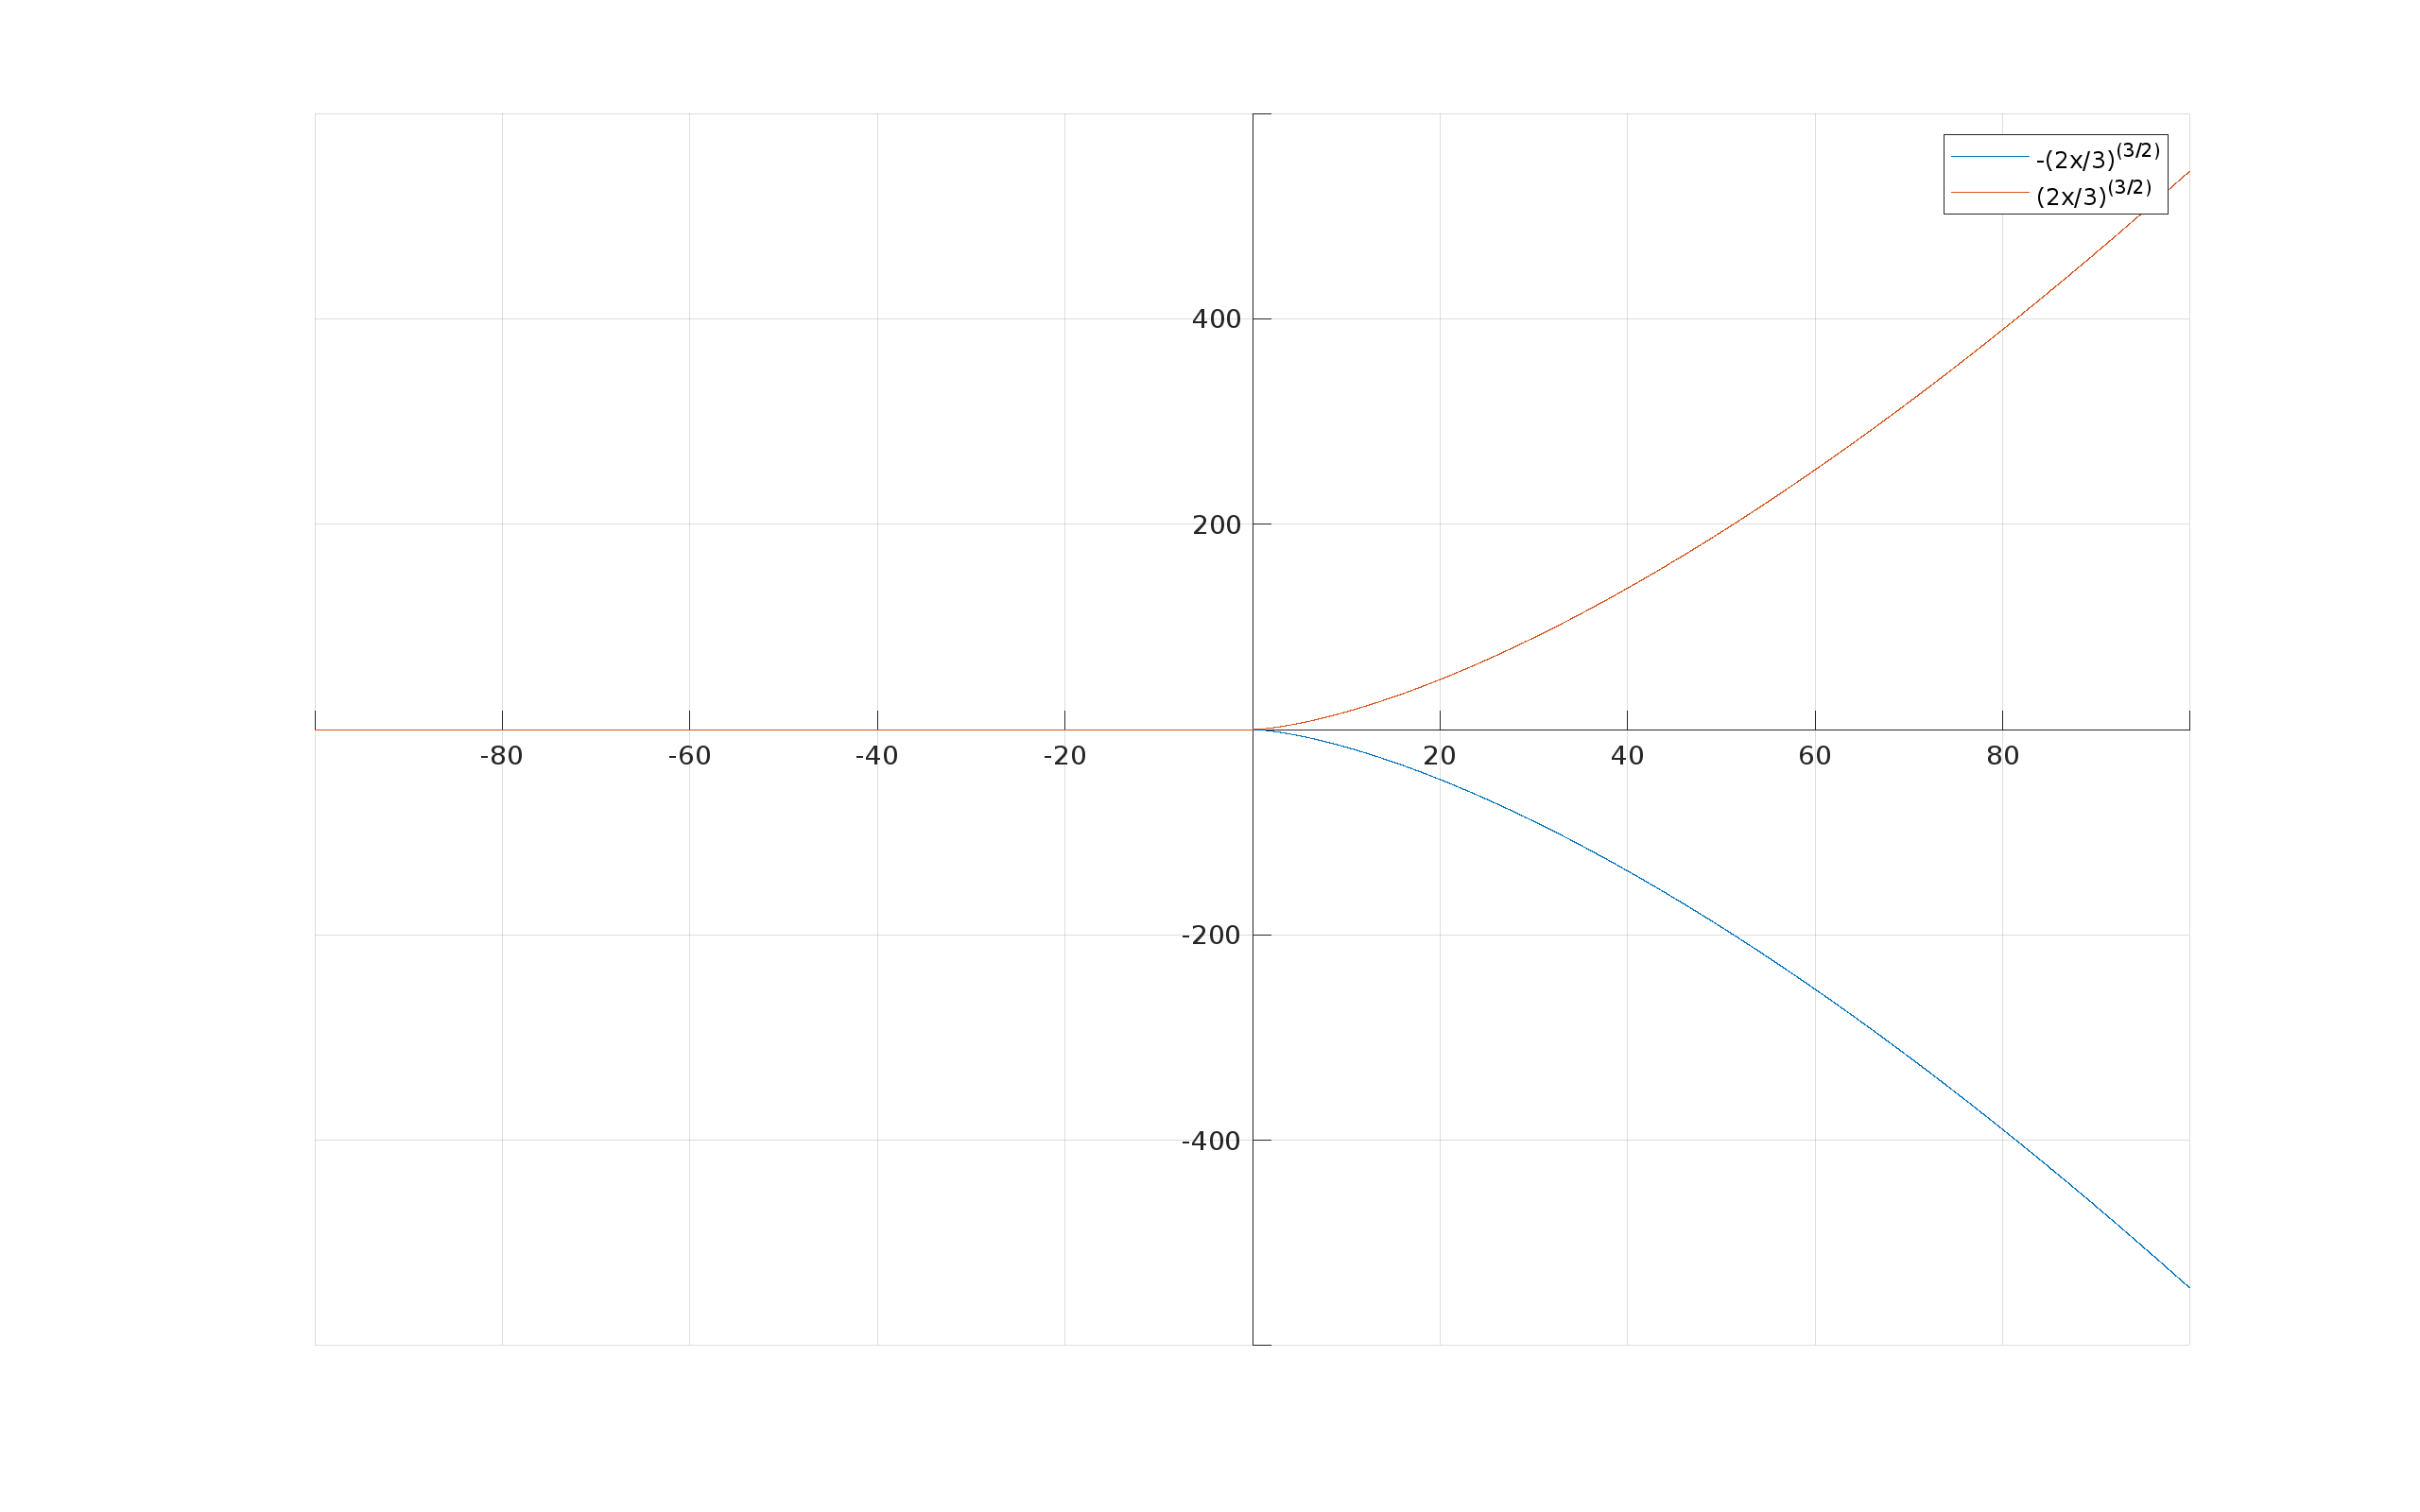
\includegraphics[width=1.0\textwidth]{Analisi2/figures/Phi.png}
    \caption{Grafico di $\varphi_2(x)=\left(\frac{2x}{3}\right)^{\frac{3}{2}}$ e $-\varphi_2(x)$.}
    \label{fig:phi}
\end{figure}

\subsubsection{EDO a variabili separabili}
\begin{definition}[EDO al primo ordine in forma normale a variabili separabili]
    \footnote{Slide 6 PDF 3.} Una EDO del primo ordine in forma normale (\ref{eq:EDO_lineare_ordine_1_forma_normale}) è detta a variabili separabili se è della forma
    \begin{equation}\label{eq:EDO_primo_ordine_forma_normale_variabili_separabili}
        y'(x) = f(x) g(y(x)),
    \end{equation}
    dove $f:I\subseteq \mathbb R\rightarrow\mathbb R,\, g: J\subseteq\mathbb R\rightarrow\mathbb R$.
\end{definition}

\paragraph{Nota:} Quando è stato trattato il problema lineare, l'equazione omogenea associata è un'equazione a variabili separabili. Si chiamano EDO a variabili separabili perché le variabili sono divise.

\paragraph{Cosa significa risolvere una EDO?} Significa trovare tutte le $y=y(x)$ definite su un opportuno intervallo per cui $y$ è derivabile e la derivata prima $y'$ verifica l'equazione (in questo caso \ref{eq:EDO_primo_ordine_forma_normale_variabili_separabili}). 

\begin{remark}
    Una EDO lineare del primo ordine omogenea in forma normale (\ref{eq:EDO_lineare_omogenea_associata_ordine_1_forma_normale}), ovvero del tipo
    \begin{equation*}
        y'(x) + a(x) y(x) = 0,
    \end{equation*}
    è a variabili separabili.
\end{remark}

\paragraph{Come si "separano" le variabili dalla equazione della forma (\ref{eq:EDO_primo_ordine_forma_normale_variabili_separabili})?} Per "separazione" delle variabili si intende la $x$ dalla $y(x)$ ed è svolta con i seguenti passaggi:
\begin{enumerate}
    \item determinare eventuali $\bar y\in\mathbb R$ [\footnotemark] per cui $g(\bar y)=0$, da cui è ottenuto
    \begin{equation}\label{eq:soluzione_EDO_variabili_separabili}
        y(x)\equiv \bar y,
    \end{equation}
    soluzione del problema. \footnote{$y(x)\equiv\bar y$ soluzione perché $g(y)=0$ e $y'=0$, dato che $\bar y$ è una funzione costante.} Inoltre, (\ref{eq:soluzione_EDO_variabili_separabili}) sono dette soluzioni singolari$_{\footnotemark}$ (o anche particolari$_{\footnotemark}$) della EDO.
    \item Considerando $y\neq\bar y$, è possibile separare le variabili dividendo per $g(y)$ (dove $g(y)\neq 0$ dato che $y\neq \bar y$, radice di $g$) la EDO, ovvero
    \begin{equation*}
        \frac{y'(x)}{g(y(x))} = \frac{f(x) \cancel{g(y(x))}}{\cancel{g(y(x))}} = f(x),
    \end{equation*}
    Da questa sono ottenute le soluzioni integrando rispetto ad $x$ ambo i membri, ovvero
    \begin{equation*}
        \int\frac{y'(x)}{g(y(x))}dx=\int f(x)dx,
    \end{equation*}
    dalle quali, ponendo $y=y(x)$ (cambiamento di variabile) e $dy = y'(x)dx$, è ottenuto
    \begin{equation*}
        \int \frac{1}{g(y)}dy = \int f(x)dx.
    \end{equation*}
    Siano $G$ e $F$ primitive di $\frac{1}{g}$ e $f$, è ottenuto
    \begin{equation*}
        G(y(x)) = F(x) + c.
    \end{equation*}
    [L'obiettivo è esplicitare $x$, quindi:] Se $G$ è invertibile si ha (la soluzione in forma implicita)
    \begin{equation*}
        y(x) = G^{-1} [F(x) + c].
    \end{equation*}
\end{enumerate}

\addtocounter{footnote}{-2}
\footnotetext{Tutte le soluzioni tali che $g(y)=0$ sono dette soluzioni singolari.}

\stepcounter{footnote}
\footnotetext{Particolari perché quando sono separate le variabili potrebbe accadere che una soluzione faccia parte dell'integrale generale per una scelta particolare della costante e quindi appartenga alla famiglia delle soluzioni.}

\stepcounter{footnote}
\footnotetext{Sono ricercati gli zeri di $g$, quindi la soluzionie di $g(y)=0$. Pertanto, data $\bar y$ soluzione (radice) del problema, con $y(x)\equiv \bar y$ soluzioni del problema, allora $g(y)=0$ (quindi $0=0$.}

\begin{example}[Esempio di applicazione del metodo precedente]\footnote{Slide 8-9 PDF 3.}
    \paragraph{Testo:} Determinare tutte le soluzioni della EDO del primo ordine (non lineare a variabili separabili)
    \begin{equation}\label{eq:esercizio_1_edo_variabili_separabili}
        y' = \underbrace{(1-y)(2-y)}_{g(y)}\underbrace{x}_{f(x)}.
    \end{equation}
    \paragraph{Svolgimento:}
    \begin{enumerate}
        \item Cerchiamo le soluzioni di $g(y)=0$, ovvero di $(1-y)(2-y) = 0$.\\
        Le soluzioni sono $y=1$ e $y=2$ (ovvero $y(x)=1$ o $y(x)=2$) e rappresentano le soluzioni costanti singolari della EDO a variabili separabili.
        \item Ora sono cercate le altre soluzioni (dividendo per $g(y)$).\\
        Data
        \begin{equation*}
            \frac{y'}{(1-y)(2-y)}=x,
        \end{equation*}
        integranado rispetto ad $x$ con cambio di variabile $y=y(x)$, è ottenuto
        \begin{equation*}
            \int \frac{y'(x)}{(1-y(x))(2-y(x))} dx = \int x\, dx.
        \end{equation*}
        Integrando con fratti semplici è ottenuto
        \begin{equation*}
            \int\frac{y'}{(1-y)(2-y)}dx = \int \frac{A}{1-y}+\frac{B}{2-y}dx,
        \end{equation*}
        dove
        \begin{equation*}
            1 = A(2-y)+B(1-y)=y(-A+B)+2A+B.
        \end{equation*}
        Tramite il principio di identità dei polinomi (Vedere Teorema \ref{th:principio_identità_polinomi})
        \begin{equation*}
            \begin{cases}
                -A-B&=0\\
                2A+B&=0
            \end{cases}\quad\Longrightarrow\quad
            \begin{cases}
                A=1\\
                B=1
            \end{cases}
        \end{equation*}
        quindi
    \begin{equation*}
        \int\frac{y'}{(1-y)(2-y)}dx \overset{y(x)=y,\, y'(x)dx=dy}{=} \int\frac{1}{1-y}dy-\int \frac{1}{2-y}dy = -\log(|1-y|) + \log(|2-y|) = \log\left|\frac{2-y}{1-y}\right|,
    \end{equation*}
    dove $y\neq 1$ (perché siamo al secondo passo).\\
    Dunque,
    \begin{equation*}
        \log\left|\frac{2-y}{1-y}\right| = \frac{x^2}{2}+c,
    \end{equation*}
    quindi
    \begin{equation*}
        \left|\frac{2-y}{1-y}\right| = \underbrace{e^{\frac{x^2}{2}+ c}}_{c_1e^{\frac{x^2}{2}}}>0.
    \end{equation*}
    Pertanto, è ottenuto che 
    \begin{equation}\label{eq:soluzioni_generali_esercizio_edo}
        \frac{2-y}{1-y}=\pm c_1 e^{\frac{x^2}{2}}=c e^{\frac{x^2}{2}},\quad c\in\mathbb R.
    \end{equation}
    \textbf{(\ref{eq:soluzioni_generali_esercizio_edo}) è la soluzione generale (anche detta "Famiglia generale"), ovvero l'integrale generale.}
    \paragraph{Intermezzo:} È necessario esprimere la soluzione generale (\ref{eq:soluzioni_generali_esercizio_edo}) in forma esplicita.\\
    Le soluzioni singolari sono $y=1$ e $y=2$. Dalla relazione (\ref{eq:soluzioni_generali_esercizio_edo}) è possibile ottenere $y=2$, ponendo $c=0$. Pertanto, la soluzione costante $y=2$ appartiene alla famiglia delle soluzioni (\ref{eq:soluzioni_generali_esercizio_edo}), con $c=0$.\\
    (\ref{eq:soluzioni_generali_esercizio_edo}) è una uguaglianza che non da la $y$ in funzione di $x$ (ciò che è ricercato), ovvero $G(x) = F(x)+c$.\\
    Alle volte le soluzioni singolari sono incluse nella famiglia generale delle soluzioni ottenuta separando le variabili, quindi al posto di unire le soluzioni ottenute dalla famiglia delle soluzioni separando le variabili e quelle singolari, è possibile ottenere le soluzioni singolari dalla (\ref{eq:soluzioni_generali_esercizio_edo}).\\
    (\ref{eq:soluzioni_generali_esercizio_edo}) è in forma implicita, quindi è necessario esplicitare la $y$ in funzione della $x$, ovvero quanto segue. $\qed$
    \begin{equation*}
        \begin{matrix}
            2-y &=& (1-y)\cdot c\cdot e^{\frac{x^2}{2}}\\
            2-y &=& ce^{\frac{x^2}{2}} - y\cdot c\cdot e^{\frac{x^2}{2}}\\
            (ce^{\frac{x^2}{2}} -1)y &=& c\cdot e^{\frac{x^2}{2}}-2 &\rightarrow& \text{non lineare.}
        \end{matrix}
    \end{equation*}
    Quindi, l'insieme delle soluzioni è dato da
    \begin{equation}\label{eq:integrale_generale_esercizio_edo_primo_ordine}
        \underbrace{y(x) = y(x,c)=\frac{c\cdot e^{\frac{x^2}{2}}-2}{c\cdot e^{\frac{x^2}{2}}-1}}_{\text{integrale generale (dipendente da $x$ e $c$)}},\quad c\in\mathbb R,
    \end{equation}
    dove $c\cdot e^{\frac{x^2}{2}}-1\neq 0$ (ovvero per tutte le $x$ dove (\ref{eq:integrale_generale_esercizio_edo_primo_ordine}) è definito).\\
    È ottenuto che:
    \begin{itemize}
        \item $y=2$ è ottenuto da (\ref{eq:integrale_generale_esercizio_edo_primo_ordine}), con $c=0$;
        \item $y=1$ non appartiene alla famiglia delle soluzioni.
    \end{itemize}
    Pertanto, \textbf{le soluzioni di (\ref{eq:esercizio_1_edo_variabili_separabili}) sono (\ref{eq:integrale_generale_esercizio_edo_primo_ordine}) e} $\boldsymbol{y=1}$. \footnote{$y=2$ appartiene già alla famiglia di soluzioni (\ref{eq:integrale_generale_esercizio_edo_primo_ordine}, quindi è esplicitato in quanto già incluso.}
    \end{enumerate}
\end{example}

\paragraph{Nota sul prossimo Esempio:} È aggiunta a (\ref{eq:integrale_generale_esercizio_edo_primo_ordine}) la condizione iniziale, ovvero: assunta una condizione iniziale, è posto il problema di Cauchy e definito qual è il più ampio intervallo sul quale è definita la soluzione. Determinare il più ampio è utile in quanto l'equazione (\ref{eq:integrale_generale_esercizio_edo_primo_ordine}) è non lineare. Pertanto, l'intervallo in questione conterrà il punto iniziale del problema ed è ricercato in modo tale che l'espressione (\ref{eq:integrale_generale_esercizio_edo_primo_ordine}) abbia senso e sia la soluzione della EDO (\ref{eq:esercizio_1_edo_variabili_separabili}).

\begin{example}[Problema di Cauchy per una EDO a variabili separabili]\footnote{Slide 11 PDF 4.}
    \paragraph{Testo:} Data la EDO del primo ordine non lineare a variabili separabili (\ref{eq:esercizio_1_edo_variabili_separabili})
    \begin{equation*}
        y' = \underbrace{(1-y)(2-y)}_{g(y)}\underbrace{x}_{f(x)},
    \end{equation*}
    con soluzioni costanti $y=1$ e $y=2$ e la soluzione generale (insieme delle soluzioni)
    \begin{equation}\label{eq:esercizio_1_intergrale_generale_problema_cauchy}
        y(x) = y(x,c)=\frac{c\cdot e^{\frac{x^2}{2}}-2}{c\cdot e^{\frac{x^2}{2}}-1},\quad c\in\mathbb R,
    \end{equation}
    con $c\cdot e^{\frac{x^2}{2}}-1\neq 0$.\\
    Risolvere il seguente problema di Cauchy (trovandone la soluzione) e specificare qual è il più ampio intervallo (rispetto all'inclusione $\subseteq$, \footnotemark) su cui è definita la soluzione,
    \begin{equation*}
        \begin{cases}
            y'&=(1-y)(2-y)x\quad\text{EDO non lineare}\\
            y(0) &= 3
        \end{cases}
    \end{equation*}
    \footnotetext{L'intervallo deve contenere il punto della condizione iniziale. Una volta definita la soluzione è necessario specificare dove è definita (su quale intervallo). Il più ampio intervallo è l'intervallo massimale rispetto all'inclusione nel quale la soluzione ha senso. È possibile osservare come le soluzioni costanti $y(x)=1$ e $y(x)=2$ non verifichino la condizione iniziale, quindi sono scartate. Ciò significa che la soluzione deve essere trovata utilizzando la formula (\ref{eq:esercizio_1_intergrale_generale_problema_cauchy}).}
    
    \paragraph{Svolgimento:} Le soluzioni $y(x)=1$ e $y(x)=2$ non verifichino la condizione iniziale, dunque è ricercata la soluzione utilizzando la formula (\ref{eq:esercizio_1_intergrale_generale_problema_cauchy}) imponendo la condizione iniziale ($y(0)=3$), ovvero
    \begin{equation*}
        3=\frac{c-2}{c-1},\quad \left(\rightarrow y(0)=\frac{ce^0-2}{ce^0-1}\right)
    \end{equation*}
    allora
    \begin{equation*}
        \begin{matrix}
            3c - 3 &=& c-2,\\
            2c &=& 1,\\
            c &=&\frac{1}{2}.
        \end{matrix}
    \end{equation*}
    La soluzione è dunque
    \begin{equation}\label{eq:soluzione_finale_esercizio_1_problema_cauchy}
        y(x)=\frac{\frac{1}{2}\cdot e^{\frac{x^2}{2}}-2}{\frac{1}{2}\cdot e^{\frac{x^2}{2}}-1} = \frac{e^{\frac{x^2}{2}}-4}{e^{\frac{x^2}{2}}-2}.
    \end{equation}
    \footnotemark L'intervallo più ampio contenente $x_0=0$, in cui la soluzione (\ref{eq:soluzione_finale_esercizio_1_problema_cauchy}) è ben definita (e contenuta) è determinata da
    \begin{equation*}
        \begin{matrix}
            e^{\frac{x^2}{2}}-2 \neq 0 &\rightarrow& e^{\frac{x^2}{2}}\neq 2 &\rightarrow& \frac{x^2}{2}\neq\ln 2 &\rightarrow& x^2\neq 2\ln2 &\rightarrow& x\neq\pm \sqrt{2\ln2}
        \end{matrix}
    \end{equation*}
    quindi l'intervallo più ampio in cui è definita la soluzione (\ref{eq:soluzione_finale_esercizio_1_problema_cauchy}) è
    \begin{equation*}
        I=(-\sqrt{2\ln2}, \sqrt{2\ln2})\ni 0.
    \end{equation*}
    \footnotetext{Affinché (\ref{eq:soluzione_finale_esercizio_1_problema_cauchy}) sia ben definito allora il denominatore di tale espressione deve essere diverso da 0.}
    
    \paragraph{Note su (\ref{eq:soluzione_finale_esercizio_1_problema_cauchy}):} è definita $\forall x\in\mathbb{R}\backslash\{\pm\sqrt{2\ln 2}\} $, ma per il problema di Cauchy richiesto di svolgere $\forall x\in I=(-\sqrt{2\ln2}, \sqrt{2\ln2})$.
    
    \paragraph{Nota su $\boldsymbol I$:} $I$ è una soluzione locale, ovvero le $x$ sono considerate vicine al punto iniziale. Quindi $y(x,c)$ è una soluzione in piccolo. Invece, se considerate le equazioni lineari ((\ref{eq:soluzione_finale_esercizio_1_problema_cauchy}) non è lineare), se i coefficienti della EDO sono continui (come nei nostri casi) la soluzione è definita in grande, ovvero su tutto l'intervallo nel quale i coefficienti della EDO sono continui.
    
    \paragraph{Nota:}
    È sbagliato affermare che la soluzione è definita $\forall x\in\mathbb R$ con $x\neq \pm\sqrt{2\log2}$ perché non è un intervallo, è ricercata la soluzione su un intervallo (ovvero un insieme limitato o illimitato contenente i punti in cui è contenuta la condizione iniziale). Affermando che $x\neq\pm\sqrt{2\log2}$ sono trovati 3 insiemi disgiunti
    \begin{equation}\label{eq:insiemi_esercizio_1_cauchy}
        (-\infty, -\sqrt{2\log2}), (-\sqrt{2\log2}, \sqrt{2\log2}), (\sqrt{2\log2}, +\infty)
    \end{equation}
    e questo non è un intervallo. Ciò ha un significato dal punto di vista fisico e matematico: dal punto di vista fisico la variabile indipendente può essere considerata come tempo, quindi è presente un sistema che evolve seguendo l'equazione differenziale definita che verifica la condizione iniziale. Quando è necessario stabilire il comportamento del sistema è controllato il comportamento in avanti (o all'indietro) partendo dal punto iniziale, dove se trovato un tempo per il quale il sistema perde di significato allora l'espressione non ha senso.\\
    Quindi, considerata la soluzione sull'intervallo è determinato l'intervallo massimale contenente la condizione iniziale.\\
    \paragraph{Significato fisico del problema di Cauchy:} La variabile indipendente può essere considerata come tempo, quindi è presente un sistema che evolve seguendo l'equazione differenziale definita che verifica la condizione iniziale. Se è trovato un tempo in cui il sistema perde significato (non esiste), non senso considerate il prima o il dopo (ad esempio $(-\infty, -\sqrt{2\log2})$ e $ (\sqrt{2\log2}, +\infty)$ in (\ref{eq:insiemi_esercizio_1_cauchy})) e quindi è considerato l'insieme massimale contente l'istante iniziale in cui il sistema fisico ha significato.
    \paragraph{Significato dal punto di vista matematico:} Dal punto di vista matematico non è possibile considerare $y(x)$ soluzione al problema di Cauchy su intervalli disgiunti come in (\ref{eq:insiemi_esercizio_1_cauchy})), perché il punto iniziale non è in $(-\infty, -\sqrt{2\log2})$ o $ (\sqrt{2\log2}, +\infty)$. Quindi la condizione iniziale determina la soluzione e l'unicità$_{\footnotemark}$ di questa nell'insieme che la contiene.
\end{example}
\footnotetext{Se considerati insiemi disgiunti, fissando la condizione iniziale, l'unicità sarebbe persa perché il punto iniziale non è in $(-\infty, -\sqrt{2\log2})$ o $ (\sqrt{2\log2}, +\infty)$.}

\begin{example}\footnote{Slide 14 PDF 4.}
    \paragraph{Testo:} Risolvere il problema di Cauchy
    \begin{equation*}
        \begin{cases}
            y' &=xy+2x\quad\text{(EDO lineare)}\\
            y(0)& = 2
        \end{cases}
    \end{equation*}
    \paragraph{Svolgimento:} Trasformazione in forma normale (ovvero $y'-a(x)y=f(x)$):
    \begin{equation*}
        y'-xy = 2x.
    \end{equation*}
    Dato che $a(x)=-x$, allora $A(x)=-\int xdx=-\frac{x^2}{2}$. Utilizzando la formula risolutiva (\ref{eq:soluzione_problema_cauchy_primo_ordine_coeff_costanti}) è ottenuto
    \begin{equation*}
        y(x) = c\cdot e^{-A(x)} + e^{-A(x)}\int f(x) e^{A(x)} dx,
    \end{equation*}
    quindi la soluzione è
    \begin{equation*}
        y(x)=y(x,c)= c\cdot e^{\frac{x^2}{2}}+ e^{\frac{x^2}{2}}\int 2xe^{-\frac{x^2}{2}}dx = c\cdot e^{\frac{x^2}{2}}+ e^{\frac{x^2}{2}}\left(-2 e^{-\frac{x^2}{2}}\right)=c\cdot e^{\frac{x^2}{2}}-2,\quad c\in\mathbb R.
    \end{equation*}
    Imponendo $y(0)=1$, allora
    \begin{equation*}
        1=c\cdot e^{0} -2\quad \rightarrow\quad c = 3,
    \end{equation*}
    quindi la soluzione è
    \begin{equation*}
        y(x) = 3e^{\frac{x^2}{2}}-2,\quad x\in\mathbb R.
    \end{equation*}
    \paragraph{Nota sulla soluzione:} In questo caso $y(x)$ è una soluzione in grande perché definita su tutta $\mathbb R$.
\end{example}

\begin{example}[Problema di Cauchy a variabili separabili]\footnote{Slide 16 PDF 4.}
    \paragraph{Testo:} Risolvere il seguente problema di Cauchy a variabili separabili
    \begin{equation*}
        \begin{cases}
            u' &= \underbrace{(1+u^2)}_{g(t)}\underbrace{\sin(t)}_{f(t)} \text{ con } u=u(t) \text{ soluzione}\\
            u(0) &= 1
        \end{cases}
    \end{equation*}
    È possibile separare le variabili a condizione che $1+u^2\neq 0$ (ovvero $u^2\geq1$). Dividendo per $g(x)$ è ottenuto
    \begin{equation*}
        \frac{u'(t)}{1+u^2(t)} = \sin t,
    \end{equation*}
    ed integrando
    \begin{equation*}
        \int \frac{u'(t)}{1+u^2(t)}dt = \int\sin t \,dt,
    \end{equation*}
    per sostituzione, con $u=u(t)$ e $dv=u'(t)\,dt$ è ottenuto che
    \begin{equation*}
        \int \frac{u'}{1+u^2}du = -\cos t + c,
    \end{equation*}
    quindi
    \begin{equation}\label{eq:arctan_esercizio_cauchy}
        \arctan u(t) = -\cos(t) + c.
    \end{equation}
    \paragraph{Intermezzo:} È possibile scrivere chi è $u(t)$. (\ref{eq:arctan_esercizio_cauchy}) è la versione implicita della soluzione, è possibile invertire la $G$, la quale è una primitiva di $\int \frac{u'}{1+u^2}du$ e quindi è utilizzata la funzione inversa (ovvero la tangente). Quindi è ottenuto quanto segue. $\qed$
    \begin{equation*}
        u(t) = \tan(-\cos t + c)= \underbrace{u(t, c)}_\text{int. gen.}\in\mathbb R.
    \end{equation*}
    Imponendo la condizione iniziale è ottenuto che
    \begin{equation*}
       \begin{matrix}
            \arctan u(0) &=& -\cos 0 + c\\
            &\Vertrarrow&\\
            \arctan 1 &=& -1 + c\\
            &\Vertrarrow&\\
            \frac{\pi}{4} &=& -1 + c\\
            &\Vertrarrow&\\
            c &=& 1+\frac{\pi}{4}
       \end{matrix}
    \end{equation*}
    Dunque la soluzione è data da
    \begin{equation*}
    	u(t)=\tan\left(-\cos t + 1 + \frac{\pi}{4}\right)\quad \forall\left(-\cos t + 1 + \frac{\pi}{4}\right)\in\left(-\frac{\pi}{2}, \frac{\pi}{2}\right).
    \end{equation*}
\end{example}

\begin{example}\footnote{Slide 16 PDF 4.}
    \paragraph{Testo:} Risolvere il problema di Cauchy
    \begin{equation*}
        \begin{cases}
            y' + 2t y^2 &= 0\\
            y(0) &= -1
        \end{cases}
    \end{equation*}
    \paragraph{Nota:} $y' + 2t y^2 = 0$ è una EDO del primo ordine non lineare a variabili separabili. Inoltre, le soluzioni sono del tipo $y=y(t)$. $\qed$\\
    Quindi,
    \begin{equation*}
        y' = -2 t y^2,
    \end{equation*}
    dove
    \begin{itemize}
        \item $f(t) = -2t$,
        \item $g(t) = y^2$,
    \end{itemize}
    entrambe funzioni definite su tutto $\mathbb R$. È possibile osservare che $y(t)=0$ è soluzione di
    \begin{equation*}
        y' + 2ty^2 = 0,
    \end{equation*}
    ma questa non verifica la condizione iniziale, quindi sono separate le variabili (dividendo per $y^2$).
    \paragraph{Nota:} È possibile dividere subito per $y^2$ in quanto la condizione $y=0$ non verifica la condizione iniziale, quindi non si puo' verificare una divisione per 0.$\qed$\\
    Data
    \begin{equation*}
    	\frac{y'(t)}{y^(t)}=2t,
    \end{equation*}
    integrando
    \begin{equation*}
    	\int\frac{y'(t)}{y^2(t)}dt=-2\int t\, dt
    \end{equation*}
    è ottenuto
    \begin{equation*}
    	-\frac{1}{y(t)} = -t^2+c,
    \end{equation*}
    ovvero
    \begin{equation*}
	\frac{1}{y(t)} = t^2-c,\quad c\in\mathbb{R}.
    \end{equation*}
    Quindi,
    \begin{equation*}
        1 = y t^2 - yc = y(t^2-c),
    \end{equation*}
    allora
    \begin{equation*}
        y(t) = \frac{1}{t^2-c}\quad\text{oppure}\quad y(t) = \frac{1}{t^2+c}.
    \end{equation*}
    (le quali sono funzioni diverse, ma l'utilizzo finale non cambia e quindi è utilizzata la forma più comoda.)
    \footnote{Per definire la soluzione è necessario che il denominatore sia diverso da 0 e ciò è legato al valore della costante. Con valori della costante positivi non ci sono problemi di definizione del dominatore, con valori negativi sono necessari esclusioni. Inoltre, è necessario trovare l'intervallo dove la soluzione e ben definita (ovvero l'intervallo contente $t=0$), quindi $t^2+c\neq 0$.}
    Imponiamo la condizione iniziale $y(0) = -1$,
    \begin{equation*}
        1=\frac{1}{0+c},
    \end{equation*}
    quindi $c=-1$. La soluzione del problema è
    \begin{equation*}
        y(t) = \frac{1}{t^2 -1},\quad \forall t\in(-1,1)\ni 0,
    \end{equation*}
    se $t^2 -1\neq 0$, ovvero $t\neq \pm 1$.
    \paragraph{Nota sulla soluzione:} La soluzione è considerata nell'intervallo massimale $(-1, 1)$ (il quale contiene $t=0$). Inoltre, l'espressione $\frac{1}{t^2 -1}$ ha senso in tutti gli intervalli in cui $t^2-1\neq 0$, ma è necessario considerare l'intervallo contenente il punto iniziale.
\end{example}

\begin{example}\footnote{Slide 19 PDF 4.}
    \paragraph{Testo:} Risolvere il problema di Cauchy
    \begin{equation*}
        \begin{cases}
            y'(x)+\frac{3x^2}{5+x^3}y(x) &= \sqrt[3]{x}\\
            y(0) &= 1
        \end{cases}
    \end{equation*}
    e precisare qual è il più ampio intervallo su cui la soluzione trovata è definita.
    \paragraph{Nota:} La EDO è lineare del primo ordine e della forma $y'+a(x)y=f(x)$, dove $a(x)=\frac{3x^2}{5+x^3}$ e $f(x) = \sqrt[3]{x}$.
    \paragraph{Svolgimento:} La EDO è definita $\forall x\in\mathbb R : x\neq-\sqrt[3]{5}$ (perché $5+x^3\neq 0$).\\
    La condizione iniziale è assegnata in $x_0=0$ e poiché $x_0>-\sqrt[3]{x}$, è considerata la soluzione sull'intervallo $I=(-\sqrt[3]{5}, +\infty)\ni 0$. \footnote{La soluzione al problema è in grande sull'intervallo.}\\
    \begin{equation*}
        A(x) = \int \frac{3x^2}{5+x^3} dx = \log(5+x^3),\quad \forall x\in I=(-\sqrt[3]{5}, +\infty),
    \end{equation*}
    quindi, l'integrale generale è
    \begin{equation*}
        \begin{matrix}
            \boldsymbol{y(x)} &=& c\cdot e^{-\log(5+x^3)} + e^{-\log(5+x^3)}\int e^{\log(5+x^3)} \sqrt[3]{x}\, dx &=& y(x,c)\\
            &=& \underbrace{\frac{1}{5+x^3}}_{\footnotemark}\left[c+\int (5+x^3)\sqrt[3]{x}dx\right] \overset{\footnotemark}{=} \frac{1}{5+x^3}\left(c+\int 5\sqrt[3]{x}dx+\int x^{\frac{10}{3}} dx\right) &=& \boldsymbol{\frac{1}{5+x^3}\left(c+5\cdot\frac{3}{4}x^{\frac{4}{3}} + \frac{3}{13}x^{\frac{13}{3}}\right)},
        \end{matrix}
    \end{equation*}
    \addtocounter{footnote}{-1}
    \footnotetext{Inversa di $e^{-\log(5+x^3)}$.}

    \stepcounter{footnote}
    \footnotetext{Linearità dell'integrale.}
    
    \noindent ovvero,
    \begin{equation*}
        y(x)= \frac{1}{5+x^3}\left(c+\cdot\frac{15}{4}x^{\frac{4}{3}} + \frac{3}{13}x^{\frac{13}{3}}\right).
    \end{equation*}
    Imponendo la condizione iniziale $y(0) = 1$ è ottenuto
    \begin{equation*}
        1=\frac{1}{5}\cdot c \quad\rightarrow\quad c=5,
    \end{equation*}
    quindi la soluzione al problema di Cauchy è
    \begin{equation*}
        y(x) = \frac{1}{5+x^3} \left(\frac{15}{4}x^{\frac{4}{3}} + \frac{3}{13}x^{\frac{13}{3}}+5\right),\quad \forall x\in(-\sqrt[3]{x}, +\infty)
    \end{equation*}
\end{example}

\begin{exercise}[Da fare a casa]
    Risolvere il problema di Cauchy
    \begin{equation*}
        \begin{cases}
            y'(x) = -\frac{\sin(2x)}{1+\cos^2(x)}y(x) + \sin x\\
            y(\pi)= 1
        \end{cases}
    \end{equation*}
    Precisare qual è il più ampio intervallo (massimale contente $\pi$) in cui la soluzione è definita.
\end{exercise}

\subsection{Risultati importanti sulle EDO del secondo ordine a coefficienti costanti}\footnote{Slide 22 PDF 4.} 
Per trovare la soluzione di questo tipo di EDO, l'integrale generale, esiste un metodo infallibile, ovvero: trovare la soluzione di un'equazione algebrica di grado 2 di campo complesso.\\
In matematica un'equazione del tipo $x^2+1=0$ non ha soluzioni in campo reale ma nel campo complesso coniugato. Quindi, affinché tale equazione abbia sempre soluzione è considerato il campo complesso. Per questo è utilizzato il Teorema \ref{th:fondamentale_algebra} fondamentale dell'Algebra (fatto a MDL o Algebra Lineare), il quale afferma che l'equazione considerata ha sempre almeno una soluzione nel campo complesso ed in particolare le soluzioni possono essere reali, distinte o coincidenti, ma se sono complesse sono complesse coniugate (intese come numeri complessi coniugati, vedere Definizione \ref{def:complesso_coniugato}).

\begin{definition}[EDO lineare del secondo ordine]\label{def:edo_lineare_secondo_ordine}
    Una EDO del secondo ordine si dice lineare se della forma
    \begin{equation}\label{eq:edo_lineare_secondo_ordine}
        a_2(x)y''(x)+a_1(x)y'(x)+a_0(x)y(x) = f(x),
    \end{equation}
    dove i coefficienti $a_i(x),\, i=0,1,2$ ed il termine noto $f(x)$ sono $C^0(I)$.
\end{definition}

\paragraph{IMPORTANTE:} Se $f(x)\neq 0$, allora (\ref{eq:edo_lineare_secondo_ordine}) è detta \textbf{completa}.

\paragraph{IMPORTANTE:} \textbf{Saranno considerate solo EDO del secondo ordine a coefficienti costanti.}

\begin{definition}[EDO lineare del secondo ordine in forma normale]
    La EDO lineare del secondo ordine (\ref{eq:edo_lineare_secondo_ordine}) è in forma normale se $a_2(x)=1$, ovvero
    \begin{equation}\label{eq:edo_lineare_secondo_ordine_forma_normale}
        y''(x)+a_1(x)y'(x)+a_0(x)y(x) = f(x).
    \end{equation}
\end{definition}

\begin{definition}[EDO lineare del secondo ordine omogenea associata]
    La EDO omogenea associata a (\ref{eq:edo_lineare_secondo_ordine}) è
    \begin{equation}\label{eq:edo_omogenea_associata_lineare_secondo_ordine}
        y''(x)+a_1(x)y'(x)+a_0(x)y(x) = 0.
    \end{equation}
\end{definition}

\paragraph{Nota:} Per la EDO completa della forma (\ref{eq:edo_lineare_secondo_ordine}) esiste l'integrale generale della forma integrale generale dell'omogenea + integrale particolare della non omogenea, ovvero il Teorema (\ref{th:rappresentazione_integrale_generale_EDO_lineare}) vale $\forall n\geq1$.

\paragraph{IMPORTANTE:} Il Teorema (\ref{th:rappresentazione_integrale_generale_EDO_lineare}) vale $\forall n\geq1$, quindi \textbf{il problema diventa trovare l'integrale generale della EDO omogenea in forma normale e l'integrale particolare della non omogenea}.

\paragraph{Rappresentazione alternativa dell'integrale generale per EDO di ordine 2:} L'integrale generale rappresentato in forma (\ref{eq:rappresentazione_integrale_generale_EDO_lineare}) può essere visto in modo informale per le EDO del secondo ordine come
\begin{equation*}
\int \text{ generale di (\ref{eq:edo_lineare_secondo_ordine_forma_normale})}=\int{\text{ generale di (\ref{eq:edo_omogenea_associata_lineare_secondo_ordine})}} + \int\text{ particolare di (\ref{eq:edo_lineare_secondo_ordine_forma_normale})}.
\end{equation*}

\begin{remark}[Non ufficiale]\label{rem:dimensione_spazio_vettoriale_edo_secondo_ordine}
    Lo spazio delle soluzioni di una EDO di ordine $n=2$ è uno spazio vettoriale di dimensione $n=2$, quindi per trovare una soluzione qualsiasi dell'omogenea servono $n=2$ soluzioni linearmente indipendenti (e da queste, com'è noto per AL, sono trovate tutte le altre).
\end{remark}

\noindent \textbf{L'Osservazione \ref{rem:dimensione_spazio_vettoriale_edo_secondo_ordine} si traduce in quanto segue:} se le funzioni $y_1(x),y_2(x)$ sono soluzioni di (\ref{eq:edo_omogenea_associata_lineare_secondo_ordine}), allora
\begin{enumerate}
    \item $y_1(x)$ e $y_2(x)$ sono linearmente indipendenti,
    \item ogni altra soluzione è una combinazione lineare di $y_1(x)$ e $y_2(x)$\footnote{Ciò segue dalla linearità della EDO, dovuto all'operatore $L$ associato ad ogni EDO lineare. $L$ è un funzionale che associa una funzione di classe $C^n(I)$ ad una funzione continua ($C^0(I)$), ovvero associa una funzione $\varphi$ a $a_n\varphi^n+\hdots+a_0\varphi^0$. Dalla linearità dell'operatore $L$ segue che se $\varphi_1$ e $\varphi_2$ sono soluzioni della EDO, anche la loro combinazione lineare è soluzione della EDO (come visto nel caso generale).}, allora \textbf{l'integrale generale generale della omogenea associata (\ref{eq:edo_omogenea_associata_lineare_secondo_ordine}) è}
    \begin{equation*}
        c_1 y_1(x) + c_2 y_2(x),
    \end{equation*}
    al variare di $c_1,c_2\in\mathbb R$.
\end{enumerate}

\paragraph{Soluzioni della omogenea associata (\ref{eq:edo_omogenea_associata_lineare_secondo_ordine}): }\footnote{Per ottenere tutte le soluzioni sono necessarie 2 soluzioni linearmente indipendenti, dato che lo spazio vettoriale di una EDO lineare omogenea ha dimensione 2. Dalle due soluzioni è costruita un sistema fondamentale di soluzioni.\\
Analogamente, per $\mathbb R^n$ la base canonica, la quale è una \gls{base ortonormale}, permette di scrivere vettori in $\mathbb R^n$ come combinazione lineare di $e_1,e_2,\hdots, e_n$. Quindi $e_1,e_2,\hdots, e_n$ formano un sistema fondamentale per lo spazio $\mathbb R^n$ perché gli elementi dello spazio sono espressi come combinazione lineare della base canonica.} Quindi, se $y_1(x)$ e $y_2(x)$ sono soluzioni linearmente indipendenti su $I$ della EDO omogenea associata (\ref{eq:edo_omogenea_associata_lineare_secondo_ordine}) (ovvero, sono la base utilizzata per scrivere una soluzione qualsiasi) allora ogni soluzione di (\ref{eq:edo_omogenea_associata_lineare_secondo_ordine}) (elemento dell'integrale generale di (\ref{eq:edo_omogenea_associata_lineare_secondo_ordine})) è una loro combinazione lineare (cioè $y_1(x)$ e $y_2(x)$ formano un sistema fondamentale di funzioni).

\footnote{Se presa una loro combinazione lineare di $y_1(x)$ e $y_2(x)$ e è posta uguale a 0, l'unica soluzione al problema è che $c_1$ e $c_2$ siano 0 $\forall x\in I$. Segue quanto scritto.} Se $y_1(x)$ e $y_2(x)$ sono soluzioni della EDO omogenea (\ref{eq:edo_omogenea_associata_lineare_secondo_ordine})) e sono linearmente indipendenti su $I$ ($\forall x\in I$), significa che
\begin{equation*}
    c_1 y_1(x) + c_2 y_2(x) = 0 \iff c_1=c_2=0.
\end{equation*}
Ciò significa che
\begin{equation}\label{eq:sistema_fondamentale_soluzioni_EDO_omogena_associata}
    \{y_1(x), y_2(x)\}
\end{equation}
formano un sistema fondamentale di soluzioni per (\ref{eq:edo_omogenea_associata_lineare_secondo_ordine}) e quindi ogni soluzione su $I$ di (\ref{eq:edo_omogenea_associata_lineare_secondo_ordine}) si scrive come loro combinazione lineare.

\paragraph{Nota su (\ref{eq:sistema_fondamentale_soluzioni_EDO_omogena_associata}):} Quanto scritto significa che l'integrale generale di una EDO del secondo ordine dipende dalle 2 costanti $c_1$ e $c_2$, oltre che dalla variabile $x$ (una EDO del primo ordine dipende da 1 costante).

\paragraph{Spiegazione di (\ref{eq:sistema_fondamentale_soluzioni_EDO_omogena_associata}):} Gli elementi di $\mathbb R^n$ sono rappresentabili tramite la base canonica (la quale è una \gls{base ortonormale}).\\
Un vettore può essere rappresentato come combinazione lineare con la base canonica, ad esempio: $(1,2)\in\mathbb R^2$ può essere espresso come $1\uline e_1 + 2\uline e_2=\uline u=(1,2)$. Lo stesso vale con (\ref{eq:sistema_fondamentale_soluzioni_EDO_omogena_associata}): $y_1(x)$ e $y_2(x)$ sono due soluzioni del problema omogeneo ed è possibile dimostrare, tramite la linearità del problema, che la loro combinazione lineare è anche la soluzione. Dato che l'obiettivo è trovare tutte le soluzioni (generare lo spazio delle soluzioni), è sufficiente avere due soluzioni indipendenti (due perché la EDO è di ordine due e lo spazio delle soluzioni è di dimensione due). La lineare indipendenza delle soluzioni sull'intervallo $I$ segue da AL:  la combinazione di $y_1(x)$ e $y_2(x)$ è linearmente indipendente (tale combinazione deve essere $=0$) se e solo se i coefficienti della combinazione sono tutti 0.\\
\textbf{Riassumendo:} Per trovare una soluzione qualsiasi del problema omogeneo (\ref{eq:edo_omogenea_associata_lineare_secondo_ordine}) è sufficiente trovare due soluzioni linearmente indipendenti del problema, le quali formano un sistema fondamentale di soluzioni.$\qed$

Data la Definizione \ref{def:edo_lineare_secondo_ordine} di EDO lineare del secondo ordine, allora è possibile la seguente.
\begin{definition}[EDO lineare del secondo ordine a coefficienti costanti]
	Una EDO lineare del secondo ordine è a coefficienti costanti se della forma
	\begin{equation}\label{eq:edo_lineare_secondo_ordine_coefficienti_costanti}
		a y'' + by' + cy =  f(x),\quad a,b,c\in\mathbb{R},\quad a\neq 0,
	\end{equation}
	dove $a=a_0(x), b=a_1(x), c=a_2(x)\in C^0(I)$ funzioni costanti e $f(x)\in C^0(I)$, con $I\subseteq\mathbb{R}$ intervallo.
\end{definition}

\begin{definition}[EDO lineare del secondo ordine omogenea a coefficienti costanti]
	Una EDO lineare del secondo ordine omogenea associata a (\ref{eq:edo_lineare_secondo_ordine_coefficienti_costanti}) è a coefficienti costanti se della forma
	\begin{equation}\label{eq:edo_lineare_secondo_ordine_omogenea_coefficienti_costanti}
		a y'' + by' + cy =  0,\quad a,b,c\in\mathbb{R},\quad a\neq 0,
	\end{equation}
	dove $a=a_0(x), b=a_1(x), c=a_2(x)\in C^0(I)$ funzioni costanti, con $I\subseteq\mathbb{R}$ intervallo.
\end{definition}

\paragraph{Considerazioni su (\ref{eq:edo_lineare_secondo_ordine_coefficienti_costanti}) e (\ref{eq:edo_lineare_secondo_ordine_omogenea_coefficienti_costanti}):}
\begin{enumerate}
	\item $a,b,c \in\mathbb{R}$ e $a\neq 0$,
	\item $x\in I$.
\end{enumerate}

\subsubsection{Ricerca dell'integrale generale \texorpdfstring{$\boldsymbol{\bar z(x)}$}{z(x)} di (\ref{eq:edo_lineare_secondo_ordine_omogenea_coefficienti_costanti})}
Per cercare la soluzione di (\ref{eq:edo_lineare_secondo_ordine_omogenea_coefficienti_costanti}) è necessario distinguere due casi:
\begin{enumerate}
	\item Se $b=c=0$ (sono identicamente nulle), l'equazione (\ref{eq:edo_lineare_secondo_ordine_omogenea_coefficienti_costanti}) diventa
	\begin{equation*}
		a y''=0,
	\end{equation*}
	quindi $y'(x)=c_1$ (è una costante). Integrando è ottenuto l'integrale generale dell'omogenea
	\begin{equation*}
		y(x)=y(x,c_1,c_2) 
		= c_1 x+c_2,\quad c_1,c_2\in\mathbb{R}.
	\end{equation*}
	\item Se $b$ e $c$ non sono identicamente nulle, per trovare l'integrale generale di (\ref{eq:edo_lineare_secondo_ordine_omogenea_coefficienti_costanti}) gli è associata una equazione algebrica di secondo grado in $\mathbb{C}$, detta equazione caratteristica di (\ref{eq:edo_lineare_secondo_ordine_omogenea_coefficienti_costanti}), della forma
	\begin{equation}\label{eq:equazione_caratteristica_associata_omogenea}
		\underbrace{a\lambda^2 + b\lambda + c}_{p(\lambda)} = 0,\quad\lambda\in\mathbb{R}.
	\end{equation}
	\footnote{L'equazione (\ref{eq:equazione_caratteristica_associata_omogenea}) è considerata in campo complesso perché $\Delta = b^2-4ac<0$, quindi le soluzioni a tale equazioni sono complesse. Per il Teorema \ref{th:fondamentale_algebra} fondamentale dell'algebra, l'equazione ha sempre due soluzioni nel campo complesso se $\Delta<0$ o reali se $\Delta>0$.} Quando $p(\lambda)=0$? Formalmente le soluzioni di (\ref{eq:equazione_caratteristica_associata_omogenea}) sono date da
	\begin{equation*}
		\lambda_{1,2} = \frac{-b\pm\sqrt{\Delta}}{2a}.
	\end{equation*}
\end{enumerate}

\begin{remark}[Non ufficiale]
	Tramite l'operatore $L$ associato alla EDO lineare omogenea di secondo grado (\ref{eq:edo_lineare_secondo_ordine_omogenea_coefficienti_costanti}), definito come 
	\begin{equation*}
		L(\varphi(x)):=a\varphi''(x) + b\varphi(x)'(x) + c\varphi(x),\quad \varphi\in C^2(I).
	\end{equation*}
	è possibile scrivere (\ref{eq:edo_lineare_secondo_ordine_omogenea_coefficienti_costanti}) come
	\begin{equation*}
		Ly(x)=0.
	\end{equation*}
	Quindi risolvere (\ref{eq:edo_lineare_secondo_ordine_omogenea_coefficienti_costanti}) significa trovare le $y$ per le quali
	\begin{equation}\label{eq:equivalenza_edo_lineare_secondo_grado_omogenea_operatore}
		(\ref{eq:edo_lineare_secondo_ordine_omogenea_coefficienti_costanti})\equiv L(y(x)) = 0.
	\end{equation}
	Inoltre, per risolvere il problema non omogoneo è posto $f(x)$ al posto di 0 in (\ref{eq:equivalenza_edo_lineare_secondo_grado_omogenea_operatore}).
\end{remark}

\begin{proposition}\footnote{Slide 3 PDF 5.}\label{prop:e^lambdax_soluzione_omogenea_secondo_grado_lineare}
	\begin{equation*}
		y(x)=e^{\lambda x}\text{ è soluzione (reale o complessa\footnotemark) di (\ref{eq:edo_lineare_secondo_ordine_omogenea_coefficienti_costanti})} \iff \lambda \text{ è radice (zero) dell'equazione } p(\lambda)=0,
	\end{equation*}
	dove $p(\lambda)=0$ è (\ref{eq:equazione_caratteristica_associata_omogenea}).
\end{proposition}
\footnotetext{Dipende da $\lambda$ se è complessa o reale.}
\begin{proof}
	È necessario dimostrare che $L(e^{\lambda x})=0\iff p(\lambda)=0$.
	\begin{equation*}
		L(e^{\lambda x}) = a(e^{\lambda x})''+ b(e^{\lambda x})'+ c e^{\lambda x} = a(\lambda^2 e^{\lambda x}) + b\lambda e^{\lambda x} + c e^{\lambda x} = e^{\lambda x} (a\lambda ^2 + b\lambda + c),
	\end{equation*}
	quindi
	\begin{equation*}
		L(e^{\lambda x}) = 0 \iff a\lambda^2 + b\lambda + c=p(\lambda) = 0.
	\end{equation*}
\end{proof}

\paragraph{Osservazione sulla dimostrazione:} Se $\lambda$ è una radice dell'equazione caratteristica associata a (\ref{eq:edo_lineare_secondo_ordine_omogenea_coefficienti_costanti}) (ovvero $\lambda$ tale che $a\lambda^2 + b\lambda + c= 0$), allora la funzione $y(\lambda)=e^{\lambda x}$ è una soluzione reale o complessa della EDO lineare omogenea di secondo ordine a coefficienti costanti (\ref{eq:edo_lineare_secondo_ordine_omogenea_coefficienti_costanti}).\\
Quindi è necessario studiare le radici (zeri) della equazione caratteristica (o equazione algebrica di secondo grado con soluzioni in $\mathbb{C}$) (\ref{eq:equazione_caratteristica_associata_omogenea}). A seconda che $\Delta$ sia $>, <$ o = 0, ci saranno due soluzioni reali distinte, due soluzioni reali coincidenti o due soluzioni complesse coniugate.

\paragraph{Determinazioni delle soluzioni linearmente indipendenti della EDO lineare omogenea di secondo ordine a coefficienti costanti (\ref{eq:edo_lineare_secondo_ordine_omogenea_coefficienti_costanti}):} Siano le due radici $\lambda_{1,2}=\frac{-b\pm\sqrt{\Delta}}{2a}$ (soluzioni del polinomio caratteristico), sono distinti i tre seguenti casi dove le soluzioni della EDO lineare omogenea di secondo ordine a coefficienti costanti (\ref{eq:edo_lineare_secondo_ordine_omogenea_coefficienti_costanti}):
\begin{enumerate}
	\item Caso $\Delta>0$:
	\begin{equation}\label{eq:soluzioni_omogenea_secondo_grado_delta_negativa}
		y_1(x) = e^{\lambda_1 x},\, y_2(x) = e^{\lambda_2 x},\quad \lambda_1,\lambda_2\in\mathbb{R}\text{ e } \lambda_1\neq\lambda_2,
	\end{equation}
	quindi l'integrale generale di (\ref{eq:edo_lineare_secondo_ordine_omogenea_coefficienti_costanti}) è
	\begin{equation*}
		\boldsymbol{\bar z(x)} = c_1 y_1(x)+ c_2y_2(x) = \boldsymbol{c_1 e^{\lambda_1 x} + c_2(x) e^{\lambda_2 x}}.
	\end{equation*}
	\item Caso $\Delta = 0$:
	\begin{equation}\label{eq:soluzioni_omogenea_secondo_grado_delta_zero}
		y_1(x) = e^{\lambda x},\, y_2(x)=x e^{\lambda x},\quad \lambda_1=\lambda_2=\lambda=\frac{-b}{2a}\in\mathbb{R},
	\end{equation}
	quindi l'integrale generale di (\ref{eq:edo_lineare_secondo_ordine_omogenea_coefficienti_costanti}) è
	\begin{equation*}
		\boldsymbol{\bar z(x) = e^{\lambda x}(c_1+c_2 x)}, 
	\end{equation*}
	\item Caso $\Delta<0$:
	\begin{equation}\label{eq:soluzioni_omogenea_secondo_grado_delta_positiva}
		y_1(x) = e^{\alpha x}\cos\beta x,\, y_2(x) = e^{\alpha x} \sin\beta x\in\mathbb{R},\quad \lambda_{1,2}=\alpha \pm i \beta\in\mathbb{C}
	\end{equation}
	dove
	\begin{itemize}
		\item $\lambda_1,\lambda_2$ soluzioni complesse del polinomio caratteristico (\ref{eq:equazione_caratteristica_associata_omogenea}) e coniugate, con $i=\sqrt{-1}$,
		\item $\alpha = -\frac{b}{2a}, \beta\overset{\footnotemark}{=}\frac{\sqrt{4ac-b^2}}{2a}\in\mathbb{R}$, parte reale dei coefficienti immaginari nei complessi con $\beta>0$ se $a>0$,
	\end{itemize}
	quindi l'integrale generale di (\ref{eq:edo_lineare_secondo_ordine_omogenea_coefficienti_costanti}) è
	\begin{equation*}
		\boldsymbol{\bar z(x) = e^{\alpha x}(c_1\cos\beta x + c_2\sin\beta x)}.
	\end{equation*}
\end{enumerate}
\footnotetext{Dato che $i=\sqrt{-1}$, allora $b^2-4ac<0$ quindi è invertito il segno di $\Delta$, ovvero $\sqrt{-\Delta}$.}

\paragraph{Cosa afferma il Teorema successivo?} Lo scopo è trovare l'integrale generale dell'EDO omogenea (\ref{eq:edo_lineare_secondo_ordine_omogenea_coefficienti_costanti}). Il Teorema successivo afferma che l'integrale generale di (\ref{eq:edo_lineare_secondo_ordine_omogenea_coefficienti_costanti}) è una combinazione lineare di $y_1$ e $y_2$. Ovvero: ogni volta che si ha a che fare l'equazione caratteristica, sono scritte le soluzioni in base a $\Delta$ e di conseguenza, trovate le soluzioni, l'integrale generale è espresso come combinazione delle soluzioni trovate. 

\begin{theorem}\footnote{Slide 5 PDF 5.}
	L'integrale generale della EDO lineare omogenea di secondo grado a coefficienti costanti (\ref{eq:edo_lineare_secondo_ordine_omogenea_coefficienti_costanti}) è data da
	\begin{equation*}
		y(x,c_1,c_2) = c_1y_1(x) + c_2y_2(x),\quad \text{ al variare dei coefficienti } c_1,c_2\in\mathbb{R},
	\end{equation*}
	dove $y_1(x)$ e $y_2(x)$ sono determinate come (\ref{eq:soluzioni_omogenea_secondo_grado_delta_positiva})-(\ref{eq:soluzioni_omogenea_secondo_grado_delta_negativa}).
\end{theorem}
\begin{proof}
	\begin{enumerate}
		\item Caso $\Delta>0$: In questo caso
		\begin{equation*}
			\Delta = b^2-4ac>0,
		\end{equation*}
		quindi $\lambda_1\neq \lambda_2$, dove $\lambda_1,\lambda_2\in\mathbb{R}$ sono soluzioni dell'equazione caratteristica (\ref{eq:equazione_caratteristica_associata_omogenea}). Dunque, per la Proposizione \ref{prop:e^lambdax_soluzione_omogenea_secondo_grado_lineare}, $e^{\lambda_1 x}$ e $e^{\lambda_2 x}$ sono soluzioni della EDO lineare omogenea di secondo grado a coefficienti costanti (\ref{eq:edo_lineare_secondo_ordine_omogenea_coefficienti_costanti}).\\
		\footnotemark (Tramite Algebra Lineare) Siano $y_1(x) = e^{\lambda_1 x}$ e $y_2(x) = e^{\lambda_2 x}$, queste sono linearmente indipendenti se
		\begin{equation*}
			\begin{matrix}
				0 &\overset{\footnotemark}{\neq}& \underbrace{\begin{vmatrix}
						y_1(x) & y_2(x)\\
						y_1'(x) & y_2'(x)
				\end{vmatrix}}_{\footnotemark} &=& y_1(x)y_2'(x) - y_2(x)y_1(x) &=&\\
				&=&
				\begin{vmatrix}
					e^{\lambda_1x} & e^{\lambda_2 x}\\
					\lambda_1 e^{\lambda_1x} & \lambda_2 e^{\lambda_2 x}
				\end{vmatrix} &=& \lambda_1 e^{(\lambda_1+\lambda_2)x} - \lambda_2 e^{(\lambda_1+\lambda_2)x} &=& (\lambda_2 -\lambda_1) e^{(\lambda_1+\lambda_2)x} &\neq& 0. 
			\end{matrix}
		\end{equation*}
		\addtocounter{footnote}{-2}
		\footnotetext{Per essere sicuri che siano generate tutte le soluzioni, quindi che è stato trovato un sistema fondamentale di soluzioni, è necessario dimostrare che le due soluzioni $y_1(x) = e^{\lambda_1 x}$ e $y_2(x) = e^{\lambda_2 x}$ siano linearmente indipendenti. È necessario ricordare che servono due elementi linearmente indipendenti per generare tutte le soluzioni perché lo spazio delle soluzioni del problema omogeneo è di dimensione 2.\\
		Quindi è necessario dimostrare che $y_1(x) = e^{\lambda_1 x}$ e $y_2(x) = e^{\lambda_2 x}$ sono linearmente indipendenti (entra in gioco Algebra Lineare). Con le mani sarà fatto vedere che la soluzione generale è una combinazione lineare di $y_1$ e $y_2$.}
		\stepcounter{footnote}
		\footnotetext{Necessario affinché $y_1$ e $y_2$ siano linearmente indipendenti.}
		\stepcounter{footnote}
		\footnotetext{Determinante della matrice Wronskiana. Una matrice Wronskiana è formata da due funzioni e dalle loro derivate prime.\\
		Considerate le soluzioni di una equazione omogenea, il determinante della Wronskiana è una funzione che dipende da $x$, se le funzioni considerate nella Wronskiana sono soluzioni del problema, il determinante è diverso da 0 e l'essere diverso da 0 indica che le funzioni sono linearmente indipendenti.}
		
		\noindent Dimostriamo (con le mani) che
		\begin{equation*}
				\begin{vmatrix}
						y_1(x) & y_2(x)\\
						y_1'(x) & y_2'(x)
				\end{vmatrix}\neq 0.
		\end{equation*} 
		Per la Proposizione \ref{prop:e^lambdax_soluzione_omogenea_secondo_grado_lineare}
		\begin{equation*}
			y_1(x) = e^{\lambda_1 x},\quad y_2(x) = e^{\lambda_2 x},
		\end{equation*}
		sono soluzioni di (\ref{eq:edo_lineare_secondo_ordine_omogenea_coefficienti_costanti}).
		\footnote{Vediamo che $y(x)$ è una soluzione qualsiasi della (\ref{eq:edo_lineare_secondo_ordine_omogenea_coefficienti_costanti}) (quindi $y(x)$ appartiene all'integrale generale di (\ref{eq:edo_lineare_secondo_ordine_coefficienti_costanti})) e che si esprime come combinazione lineare di $y_1(x)$ e $y_2(x)$. Ovvero, lo scopo è far vedere che $y(x)=c_1 e^{\lambda_1x}+c_2e^{\lambda_2 x}=(\ref{eq:integrale_generale_secondo_ordine_dimostrazione})$.} Sia $y(x)$ soluzione di  (\ref{eq:edo_lineare_secondo_ordine_omogenea_coefficienti_costanti}), scriviamo tale funzione come
		\begin{equation}\label{eq:integrale_generale_secondo_ordine_dimostrazione}
			y(x) = e^{\lambda_2 x}\underset{\footnotemark}{u(x)}
		\end{equation}
		\footnotetext{Funzione opportuna e non costante, da determinare affinché $y(x)$ sia soluzione di (\ref{eq:edo_lineare_secondo_ordine_omogenea_coefficienti_costanti}).}
		Poiché $y(x)$ è soluzione di  (\ref{eq:edo_lineare_secondo_ordine_omogenea_coefficienti_costanti}) (e ciò significa che verifica la EDO), si ha che
		\begin{equation*}
			a(e^{\lambda_1x}u(x))''+ b(e^{\lambda_1x}u(x))'+ c (e^{\lambda_1x}u(x)) = 0.
		\end{equation*}
		È necessario verificare quanto appena scritto] Dunque
		\begin{equation}\label{eq:dimostrazione_th_soluzioni_edo_secondo_ordine}
			\begin{matrix}
				a(\lambda_1e^{\lambda_1x}u(x)+e^{\lambda_1x}u'(x))' + b(\lambda_1 e^{\lambda_1 x}u(x) + e^{\lambda_1x}u'(x)) + c(e^{\lambda_1x}u(x)) &=&\\\\
				a(\lambda_1^2e^{\lambda_1 x}u(x) + 2 e^{\lambda_1 x} u'(x) + e^{\lambda_1 x}u''(x))+ b (\lambda_1 e^{\lambda_1 x}u(x) + e^{\lambda_1 x}u'(x)) + x
				c(e^{\lambda_1 x}u(x)) &=&\\\\
				 \underbrace{e^{\lambda_1 x}}_{>0} [\underbrace{(a\lambda_1^2+b\lambda_1 +c) u(x)}_{0} + a u''(x)+(2a\lambda_1 + b)u'(x)] &\underset{\footnotemark}{=}& 0
			\end{matrix}
		\end{equation}
		\footnotetext{L'equazione è 0 s.se a sinistra, ciò che è fra parentesi quadre è 0.}
		\hrule\vspace{-12px}
		\paragraph{Osservazioni (intermezzo):}
		\begin{enumerate}
			\item È noto che $\lambda_1$ è soluzione dell'equazione caratteristica $p(\lambda_1)=0$, ovvero di $(a\lambda_1^2+b\lambda_1 +c)$. Quindi, rimane da dimostrare che $a u''(x)+(2a\lambda_1 + b)u'(x)$ sia 0;
			\item l'equazione caratteristica è $a\lambda_1^2+b\lambda_1 +c$, quindi (dato che $a\neq0$, altrimenti la EDO non sarebbe di secondo grado)
			\begin{equation*}
				\lambda + \frac{b}{a} \lambda + \frac{c}{a}= (\lambda - \lambda_1)(\lambda - \lambda_2) = 0,
			\end{equation*}
			dove
			\begin{equation}\label{eq:lambda1_+_lambda2}
				\lambda_1 + \lambda_2 = \frac{-b}{a}
			\end{equation}
			\begin{equation*}
				\lambda_1 - \lambda_2 = \frac{c}{a}
			\end{equation*}
		\end{enumerate}
		\hrule\vspace{2px}
		Cerchiamo di riscrivere
		\begin{equation*}
			a u''(x)+(2a\lambda_1 + b)u'(x)=0.
		\end{equation*}
		Dividendo per $a$ è ottenuto (il caso (\ref{eq:lambda1_+_lambda2}), ovvero)
		\begin{equation*}
			u''(x)+\left(2\lambda_1+\frac{b}{a}\right)u'(x)=0,
		\end{equation*}
		quindi (sostituendo),
		\begin{equation*}
			u''(x) + (2\lambda_1 -\lambda_1+\lambda_2) u'(x) = 0,
		\end{equation*}
		ovvero
		\begin{equation*}
			u''(x) - \underbrace{(\lambda_2-\lambda_1)}_{k\neq 0\text{ costante}} u'(x) = 0.\quad\text{(La quale è una EDO del seguente tipo)}.
		\end{equation*}
		Pertanto,
		\begin{equation*}
			u''(x)- u'(x) = 0,
		\end{equation*}
		con $u'(x)=v(x)$, diventa
		\begin{equation}\label{eq:edo_variabili_separabili_dimostrazione_integrale_generale_edo_seecondo_grado}
			v'(x) - k \cdot v(x)=0,
		\end{equation}
		la quale ha soluzione (esponenziale)
		\begin{equation*}
			v(x) = c \cdot e^{kx}.
		\end{equation*}
		\footnote{(\ref{eq:edo_variabili_separabili_dimostrazione_integrale_generale_edo_seecondo_grado}) è a variabili separabili. Dato che $v(x)=u'(x)$, allora $u'(x)=ce^{(\lambda_2-\lambda_1)x}$ e $v(x)=ce^{(\lambda_2-\lambda_1)x}$. Quindi è possibile integrare, tenendo di conto che $e^{(\lambda_2-\lambda_1)x}$ è un esponenziale è necessaria una correzione del coefficiente $c$ affinché $\lambda_1-\lambda_2\neq 0$. Ciò non è scritto esplicitamente, è denotata una costante $c_1=\frac{c}{\lambda_2-\lambda_1}$ tale che $u(x) = c_1 e^{\lambda_1-\lambda_2}$. Quanto descritto è formalizzato in seguito alla nota.} Integrando
		\begin{equation*}
			u'(x)=c\cdot e^{(\lambda_2-\lambda_1)x},\quad u(x)=\int u'(x)\,dx,
		\end{equation*}
		è ottenuto
		\begin{equation*}
			u(x)=\underset{\footnotemark}{c_1}\cdot e^{(\lambda_2-\lambda_1)x}+\underset{\boldsymbol{\footnotemark}}{c_2},\quad c_1,c_2\in\mathbb{R},
		\end{equation*}
		essendo
		\begin{equation*}
			y(x)=e^{\lambda_1 x}u(x)\overset{\text{sost.}}{=}e^{\lambda_1x}\left[c_1\cdot e^{(\lambda_2-\lambda_1)x}+c_2\right] = c_1\cdot e^{\lambda_2 x} + c_2\cdot e^{\lambda_1 x}
		\end{equation*}
		\footnotetext{È necessario modificare la costante $c$: $c_1$ è collegata al fattore connettivo da utilizzare quando è calcolata una primitiva di un esponenziale del tipo $e^{(\lambda_2-\lambda_1)x}$. In particolare $c$ deve essere diviso per $\lambda_1-\lambda_2$. $c_1$ è collegato a $k$ in (\ref{eq:edo_variabili_separabili_dimostrazione_integrale_generale_edo_seecondo_grado}).}
		\footnotetext{Necessaria per comprendere tutte le soluzioni.}
		\item \textbf{Caso $\boldsymbol{\Delta=0}$:} In questo caso
		\begin{equation*}
			\lambda_1=\lambda_2=\lambda=\frac{-b}{2a},
		\end{equation*}
		dunque le soluzione di (\ref{eq:edo_lineare_secondo_ordine_omogenea_coefficienti_costanti})
		\begin{equation*}
			y_1(x)=e^{\lambda_1 x},\quad y_2(x) = e^{\lambda_2 x},
		\end{equation*}
		possono essere denotate come
		\begin{equation*}
			y(x) = e^{\lambda x}.
		\end{equation*}
		\hrule\vspace{-2px}
		È necessario mostrare che ogni soluzione è combinazione lineare di $y_1$ e $y_2$ e per farlo è seguita la procedura del precedente caso: è stabilito se sono linearmente indipendenti mediante il determinante della matrice Wronskiana. Inoltre, c'è una soluzione $\lambda$ se $p(\lambda)=0$.
		\hrule\vspace{2px}
		
		\noindent Data $y(x) = e^{\lambda x}$, questa è linearmente indipendente se
		\begin{equation*}
			\begin{vmatrix}
				e^{\lambda x} & e^{\lambda x}\\
				\lambda e^{\lambda x} & \lambda  e^{\lambda  x} + \lambda x e^{\lambda x}
			\end{vmatrix} =  \begin{vmatrix}
				e^{\lambda x} & e^{\lambda  x}\\
				\lambda  e^{\lambda x} & \lambda  e^{\lambda  x} (1 + \lambda x e^{\lambda x})
			\end{vmatrix}\neq 0.
		\end{equation*}
		(Provato che $y$ è linearmente indipendenti)\\
		Sia $y(x)$ soluzione qualsiasi di (\ref{eq:edo_lineare_secondo_ordine_omogenea_coefficienti_costanti}) della forma 
		\begin{equation*}
			y(x) = e^{\lambda x} u(x),
		\end{equation*}
		allora (procedendo come prima, poiché $y(x)$ è una soluzione di (\ref{eq:edo_lineare_secondo_ordine_omogenea_coefficienti_costanti}))
		\begin{equation*}
			a(e^{\lambda x}u(x))'' + b(e^{\lambda x} u(x))' + c e^{\lambda x} u(x) =0,
		\end{equation*}
		dunque è ottenuto [come in per (\ref{eq:dimostrazione_th_soluzioni_edo_secondo_ordine})]
		\begin{equation*}
			\begin{matrix}
				a(\lambda e^{\lambda x}u(x)+e^{\lambda x}u'(x))' + b(\lambda e^{\lambda x}u(x) + e^{\lambda x}u'(x)) + c(e^{\lambda x}u(x)) &=&\\\\
				\underbrace{e^{\lambda x}}_{>0} [\underbrace{(a\lambda^2+b\lambda +c) u(x)}_{0} + a u''(x)+(2a\lambda + b)u'(x)] &=& 0.
			\end{matrix}
		\end{equation*}
		Cerchiamo di scrivere
		\begin{equation*}
			a u''(x)+(2a\lambda + b)u'(x)=0.
		\end{equation*}
		Dividendo per $a$ è ottenuto (il caso (\ref{eq:lambda1_+_lambda2}), ovvero)
		\begin{equation*}
			u''(x)+(2\lambda + \frac{b}{a})u'(x).
		\end{equation*}
		dove $2\lambda = -\frac{b}{a}$ e $u''(x)=0$.
		Quindi, integrando
		\begin{equation*}
			u(x) = c_1+c_2 x,
		\end{equation*}
		e dunque
		\begin{equation*}
			y(x) = e^{\lambda x}u(x) = e^{\lambda x} (c_1+c_2x) = c_1\cdot \underbrace{e^{\lambda x}}_{y_1(x)} + c_2\cdot\underbrace{x\cdot e^{\lambda x}}_{y_2(x)}.
		\end{equation*}
	\end{enumerate}
\end{proof}

\subsection{Cose non fatte ma utili}
\begin{theorem}[Principio di identicità dei polinomi]\label{th:principio_identità_polinomi}
		Due polinomi ridotti in forma normale sono identici, ovvero
		\begin{equation*}
			a_nx^n+a_{n-1}x^{n-1}+\hdots+a_0x^0 = b_nx^n+b_{n-1}x^{n-1}+\hdots+b_0x^0,
		\end{equation*}
		se hanno lo stesso grado $n$ e gli stessi coefficienti nei termini di grado uguale, ovvero se
		\begin{equation*}
			a_i=b_i\quad\forall i\in(0,1,\hdots, n).
		\end{equation*}
\end{theorem}
\paragraph{Esempio pratico del Teorema \ref{th:principio_identità_polinomi}:} Siano $A,B,C$ parametri e i \gls{polinomi}
\begin{equation*}
	\begin{matrix}
		P(x) &=& x^3 + 4x^2-x+1\\
		Q(x) &=& Cx^4 + (A+B)x^3+2Ax^2-x+1
	\end{matrix}
\end{equation*}
Per quali valori dei parametri i due polinomi sono identici?\\
È necessario imporre che
\begin{equation*}
	\begin{cases}
		C&=0\\
		A+B &= 1\\
		2A &= 4
	\end{cases}
\end{equation*}
da cui, è ottenuto
\begin{equation*}
	\begin{cases}
		A &= 2\\
		B &= - 1\\
		C&=0
	\end{cases}
\end{equation*}

\begin{theorem}[Teorema fondamentale dell'algebra]\label{th:fondamentale_algebra}
   Ogni polinomio in una variabile di grado $n\geq 1$ (cioè non costante) con coefficienti complessi, del tipo
    \begin{equation*}
        a_{n}z^{n}+\ldots +a_{1}z+a_{0},
    \end{equation*}
    ammette almeno una radice complessa (o zero). 
\end{theorem}
\begin{definition}[Numero complesso]
    Dati $x,y\in\mathbb R$ e $i\in\mathbb C$ (detta unità immaginaria) soluzione dell'equazione $x^2=-1$, un numero complesso è definito come
    \begin{equation*}
        z=x+iy.
    \end{equation*}
\end{definition}
Un numero complesso coniugato di un numero complesso è il numero ottenuto dal primo cambiando di segno alla parte immaginaria.
\begin{definition}[Numero complesso coniugato]\label{def:complesso_coniugato}
    Dato il numero complesso
    \begin{equation*}
        z = x + i y,
    \end{equation*}
    dove $x$ e $y$ sono numeri reali ed $i$ è l'unità immaginaria, il complesso coniugato di $z$ si indica con $\bar {z}$ ed è definito da
    \begin{equation*}
        \bar {z}=x-iy.
    \end{equation*}
\end{definition}

\begin{definition}[Applicazione Lineare]\label{def:applicazione_lineare}
	Siano $A$ e $B$ due spazi vettoriali definiti sullo stesso campo $C$. Una funzione $f:A\rightarrow B$ è un'\gls{applicazione lineare} se soddisfa le seguenti proprietà $\forall x,y\in A$ e $\forall a\in C$:
	\begin{enumerate}
		\item $f(x+y)=f(x)+f(y),$
		\item $f(\alpha x)=\alpha f(x)$.
	\end{enumerate}
\end{definition}

\subsection{Metodo di somiglianza}\label{ssec:metodo_somiglianza}
DA INSERIRE

\subsection{Variazione delle costanti}\label{ssec:variazione_costanti}